\documentclass[11pt,a4paper,oneside]{report}

% ============================================================
% PACKAGES
% ============================================================
\usepackage[utf8]{inputenc}
\usepackage[T1]{fontenc}
\usepackage{lmodern}
\usepackage[margin=2.35cm,headheight=28pt]{geometry}
\usepackage[table]{xcolor}
\usepackage{colortbl}
\usepackage{titlesec}
\usepackage{fancyhdr}
\usepackage[most]{tcolorbox}
\tcbuselibrary{skins,breakable,listings}
\usepackage{listings}
\usepackage{enumitem}
\usepackage{hyperref}
\usepackage{bookmark}
\usepackage{tikz}
\usetikzlibrary{arrows.meta,positioning,fit,shapes.geometric,calc}
\usepackage{tabularx}
\usepackage{booktabs}
\usepackage{graphicx}
\usepackage{lastpage}
\usepackage{sectsty}
\usepackage[most]{tcolorbox}
\usepackage{longtable}
\usepackage{array}
\usepackage{ragged2e}
\usepackage{float}
\usepackage{microtype}
\usepackage{multicol}
\usepackage{etoolbox}
\usepackage{pifont}
\usepackage{setspace}

% ============================================================
% DOCUMENT METADATA
% ============================================================
\newcommand{\DocumentTitle}{LINC Ministry Portal}
\newcommand{\DocumentSubtitle}{Current-State Technical Assessment, Target Architecture, and Enterprise Modernization Plan}
\newcommand{\DocumentVersion}{1.2}
\newcommand{\DocumentStatus}{Architecture Baseline, Implemented Backend Slice, and Modernization Specification}
\newcommand{\DocumentAuthor}{Kirolos Sedra}
\newcommand{\DocumentAffiliation}{T-TLabs / LINC Ministry}
\newcommand{\DocumentClassification}{Confidential -- Internal Use Only}

% ============================================================
% COLOR PALETTE
% ============================================================
\definecolor{primary}{HTML}{1B3A6B}
\definecolor{secondary}{HTML}{2E86AB}
\definecolor{accent}{HTML}{F2A541}
\definecolor{lightgray}{HTML}{F4F6F8}
\definecolor{midgray}{HTML}{6E7B8B}
\definecolor{darkgray}{HTML}{344054}
\definecolor{codebg}{HTML}{F7F9FB}
\definecolor{notegreen}{HTML}{2E7D32}
\definecolor{warnred}{HTML}{C62828}
\definecolor{criticalred}{HTML}{8E1B1B}
\definecolor{purple}{HTML}{6B4E9B}

% ============================================================
% GENERAL TYPOGRAPHY
% ============================================================
\setlength{\parindent}{0pt}
\setlength{\parskip}{6pt}
\setlength{\emergencystretch}{2em}
\renewcommand{\arraystretch}{1.22}
\setlist[itemize]{leftmargin=1.6em,itemsep=3pt,topsep=4pt}
\setlist[enumerate]{leftmargin=1.8em,itemsep=3pt,topsep=4pt}

% ============================================================
% SECTION STYLING
% ============================================================
\titleformat{\chapter}[display]
  {\normalfont\huge\bfseries\color{primary}}
  {\filright\Large\color{secondary}\chaptertitlename\ \thechapter}
  {8pt}{\Huge}
\titlespacing*{\chapter}{0pt}{0pt}{24pt}

\titleformat{\section}
  {\normalfont\Large\bfseries\color{primary}}
  {\thesection}{10pt}{}
\titleformat{\subsection}
  {\normalfont\large\bfseries\color{secondary}}
  {\thesubsection}{8pt}{}
\titleformat{\subsubsection}
  {\normalfont\normalsize\bfseries\color{darkgray}}
  {\thesubsubsection}{7pt}{}

% ============================================================
% HEADER / FOOTER
% ============================================================
\pagestyle{fancy}
\fancyhf{}
\renewcommand{\headrulewidth}{0.6pt}
\renewcommand{\footrulewidth}{0.4pt}
\fancyhead[L]{\small\color{midgray}\textsc{\DocumentTitle}}
\fancyhead[R]{\small\color{midgray}\nouppercase{\leftmark}}
\fancyfoot[L]{\small\color{midgray}Prepared by \DocumentAuthor}
\fancyfoot[R]{\small\color{midgray}Page \thepage\ of \pageref{LastPage}}

\fancypagestyle{plain}{
  \fancyhf{}
  \fancyfoot[C]{\small\color{midgray}Page \thepage\ of \pageref{LastPage}}
  \renewcommand{\headrulewidth}{0pt}
}

% ============================================================
% HYPERLINK STYLING
% ============================================================
\hypersetup{
  colorlinks=true,
  linkcolor=secondary,
  urlcolor=accent!80!black,
  citecolor=secondary,
  pdftitle={\DocumentTitle: \DocumentSubtitle},
  pdfauthor={\DocumentAuthor},
  pdfsubject={Enterprise software architecture and modernization documentation},
  pdfkeywords={LINC, ministry portal, React, Firebase, backend architecture, security, modernization},
}

% ============================================================
% CODE LISTING STYLE
% ============================================================
\lstdefinelanguage{TypeScript}{
  keywords={const,let,var,function,return,if,else,for,while,async,await,interface,type,export,import,from,class,extends,implements,private,public,protected,new,try,catch,finally,true,false,null,undefined},
  sensitive=true,
  comment=[l]{//},
  morecomment=[s]{/*}{*/},
  morestring=[b]',
  morestring=[b]"
}

\lstdefinestyle{codestyle}{
  backgroundcolor=\color{codebg},
  commentstyle=\color{midgray}\itshape,
  keywordstyle=\color{primary}\bfseries,
  numberstyle=\tiny\color{midgray},
  stringstyle=\color{notegreen},
  basicstyle=\ttfamily\footnotesize,
  breaklines=true,
  numbers=left,
  numbersep=8pt,
  frame=single,
  rulecolor=\color{midgray!40},
  tabsize=2,
  showstringspaces=false,
  columns=fullflexible,
}
\lstset{style=codestyle}

% ============================================================
% CUSTOM BOXES
% ============================================================
\newtcolorbox{infobox}[1][]{
  breakable, enhanced, colback=secondary!6, colframe=secondary,
  boxrule=0.8pt, arc=2pt, left=8pt, right=8pt, top=6pt, bottom=6pt,
  title={Info #1},
  fonttitle=\bfseries\color{white},
  colbacktitle=secondary,
}

\newtcolorbox{notebox}[1][]{
  breakable, enhanced, colback=notegreen!6, colframe=notegreen,
  boxrule=0.8pt, arc=2pt, left=8pt, right=8pt, top=6pt, bottom=6pt,
  title={Note #1},
  fonttitle=\bfseries\color{white},
  colbacktitle=notegreen,
}

\newtcolorbox{warningbox}[1][]{
  breakable, enhanced, colback=warnred!6, colframe=warnred,
  boxrule=0.8pt, arc=2pt, left=8pt, right=8pt, top=6pt, bottom=6pt,
  title={Warning #1},
  fonttitle=\bfseries\color{white},
  colbacktitle=warnred,
}

\newtcolorbox{taskbox}[1][]{
  breakable, enhanced, colback=accent!10, colframe=accent!80!black,
  boxrule=0.8pt, arc=2pt, left=8pt, right=8pt, top=6pt, bottom=6pt,
  title={Task #1},
  fonttitle=\bfseries\color{black},
  colbacktitle=accent,
}

\newtcolorbox{criticalbox}[1][]{
  breakable, enhanced, colback=criticalred!5, colframe=criticalred,
  boxrule=1.0pt, arc=2pt, left=8pt, right=8pt, top=6pt, bottom=6pt,
  title={Critical #1},
  fonttitle=\bfseries\color{white},
  colbacktitle=criticalred,
}

\newtcolorbox{decisionbox}[1][]{
  breakable, enhanced, colback=purple!6, colframe=purple,
  boxrule=0.8pt, arc=2pt, left=8pt, right=8pt, top=6pt, bottom=6pt,
  title={Architecture Decision #1},
  fonttitle=\bfseries\color{white},
  colbacktitle=purple,
}

\newtcolorbox{paramtable}[1][]{
  breakable, enhanced, colback=lightgray, colframe=primary!70,
  boxrule=0.6pt, arc=2pt, left=6pt, right=6pt, top=6pt, bottom=6pt,
  title=#1, fonttitle=\bfseries\color{white}, colbacktitle=primary,
}

% ============================================================
% STATUS COMMANDS
% ============================================================
\newcommand{\statusactive}{\textcolor{notegreen}{\textbf{ACTIVE}}}
\newcommand{\statusrefactor}{\textcolor{accent!80!black}{\textbf{REFACTOR}}}
\newcommand{\statusremove}{\textcolor{warnred}{\textbf{REMOVE}}}
\newcommand{\statusnew}{\textcolor{secondary}{\textbf{NEW}}}
\newcommand{\statusverify}{\textcolor{purple}{\textbf{VERIFY}}}
\newcommand{\yes}{\textcolor{notegreen}{\ding{51}}}
\newcommand{\no}{\textcolor{warnred}{\ding{55}}}

% ============================================================
% DOCUMENT
% ============================================================
\begin{document}

% ---------------- TITLE PAGE ----------------
\begin{titlepage}
\begin{tikzpicture}[remember picture, overlay]
  \fill[primary] (current page.north west) rectangle ([yshift=-3.1cm]current page.north east);
  \fill[accent] ([xshift=0.12\paperwidth,yshift=-3.1cm]current page.north west) rectangle ([yshift=-3.22cm]current page.north east);
  \fill[secondary!15] (current page.south west) rectangle ([yshift=1.2cm]current page.south east);
\end{tikzpicture}

\vspace*{4.35cm}
\begin{center}
  {\color{primary}\rule{0.72\textwidth}{1.2pt}}\\[0.55cm]
  {\Huge\bfseries\color{primary} \DocumentTitle}\\[0.35cm]
  {\Large\color{secondary} \DocumentSubtitle}\\[0.55cm]
  {\color{primary}\rule{0.72\textwidth}{1.2pt}}\\[2.1cm]

  {\large\textsc{Version \DocumentVersion}}\\[0.25cm]
  {\large \today}\\[2.4cm]

  \begin{tabular}{>{\bfseries}rl}
    Author: & \DocumentAuthor \\
    Affiliation: & \DocumentAffiliation \\
    Document status: & \DocumentStatus \\
    Classification: & \DocumentClassification \\
  \end{tabular}
\end{center}

\vfill
\begin{center}
  \small\color{midgray}
  This document records the actual reviewed implementation, identifies architectural and security weaknesses, and defines the target enterprise architecture and migration program.
\end{center}
\end{titlepage}

% ---------------- DOCUMENT CONTROL ----------------
\chapter*{Document Control}
\addcontentsline{toc}{chapter}{Document Control}

\begin{paramtable}[Document Information]
\begin{tabularx}{\linewidth}{@{}>{\bfseries}l X@{}}
\toprule
Title & \DocumentTitle: \DocumentSubtitle \\
Version & \DocumentVersion \\
Status & \DocumentStatus \\
Owner & \DocumentAuthor \\
Classification & \DocumentClassification \\
Primary audience & Product owner, software engineers, security reviewers, ministry leadership, administrators, maintainers, and prospective implementation partners \\
Review basis & Source-code inspection of the provided React, Firebase, YAML, service, and page modules, supplemented by confirmed operational requirements and modernization decisions \\
\bottomrule
\end{tabularx}
\end{paramtable}

\begin{table}[H]
\centering
\rowcolors{2}{lightgray}{white}
\begin{tabularx}{\linewidth}{@{}l l l X@{}}
\toprule
\rowcolor{primary}
\textcolor{white}{\textbf{Version}} & \textcolor{white}{\textbf{Date}} & \textcolor{white}{\textbf{Author}} & \textcolor{white}{\textbf{Change Summary}} \\
\midrule
1.2 & July 24, 2026 & \DocumentAuthor & Documented the implemented Cloudflare Worker backend foundation and the completed participant meeting-invitation migration from browser-side EmailJS to authenticated backend Brevo delivery, including Hono routing, Zod validation, Firebase ID-token verification, bilingual email generation, Worker secrets, CORS, Vitest tests, GitHub Actions, Netlify secret-scan remediation, separate frontend/backend deployment, production troubleshooting, current limitations, and skills learned. \\
1.1 & July 22, 2026 & \DocumentAuthor & Added the implemented landing-page floating action dock: scroll-triggered promotion of hero actions, viewport-safe responsive layout, return animation, reduced-motion behavior, and related testing and acceptance requirements. \\
1.0 & July 22, 2026 & \DocumentAuthor & Initial enterprise documentation baseline covering current-state analysis, target architecture, security model, migration plan, and delivery roadmap. \\
\bottomrule
\end{tabularx}
\caption{Document revision history}
\end{table}

\begin{warningbox}[-- Controlled Baseline]
This document is an architecture and modernization baseline. It deliberately describes the existing implementation candidly. The Cloudflare Worker backend foundation and participant meeting-invitation migration documented in the implemented-backend chapter are completed current-state work supported by code, tests, and deployment evidence. The broader target architecture, role model, database migration, and enterprise controls remain recommendations until separately verified through code, infrastructure, tests, and deployment evidence.
\end{warningbox}

% ---------------- TOC ----------------
\pagestyle{plain}
\tableofcontents
\clearpage
\listoffigures
\clearpage
\listoftables
\clearpage
\pagestyle{fancy}

% ============================================================
\chapter{Executive Summary}
% ============================================================

\section{Project Assessment}

The LINC Ministry Portal has evolved from a bilingual spiritual-gifts assessment into a broad ministry operations platform. Its current feature set includes configurable assessments, public meeting requests, Pastor calendar management, NextGen participation, attendance tracking, People Development groups, confidential pastoral notes, bilingual presentation, email notifications, and several administrative functions.

The implementation demonstrates substantial product discovery and domain knowledge. It also contains several useful transactional ideas, such as Firebase transactions for unique NextGen identifiers and voting. The landing page now additionally includes a responsive, scroll-aware floating action dock that preserves access to the six primary actions after the original hero buttons leave the viewport and restores the normal layout when the user scrolls back to the top.

A first production backend slice has now been implemented. A Cloudflare Worker using Hono, TypeScript, Zod, and \texttt{jose} receives authenticated participant meeting-invitation requests from the React frontend, validates the payload, generates bilingual English/Arabic email content, and calls Brevo using a Worker-side secret. The frontend continues to use its existing Firebase Authentication session, so no additional login screen or pastor-facing authentication step was introduced. Vitest tests and GitHub Actions protect the backend foundation, while Netlify and Cloudflare Workers remain separate deployment surfaces.

\begin{criticalbox}[-- Primary Architectural Finding]
The application is now a hybrid system rather than a completely two-tier application: participant meeting invitations use a protected backend path, but most domains still read and write Firebase or invoke legacy providers directly from the browser. The remaining direct-client access model is not suitable as the long-term architecture for confidential pastoral records, attendance history, participant identities, administrative permissions, booking decisions, and other sensitive workflows.
\end{criticalbox}

The central modernization direction remains:

\begin{center}
\textbf{Frontend $\rightarrow$ Backend/API $\rightarrow$ Database and External Services}
\end{center}

The implemented invitation service proves this migration pattern in production. The backend must progressively become the authoritative enforcement and orchestration layer for authorization, validation, transactions, privacy boundaries, notifications, audit logging, rate limiting, file handling, and migrations. This direction aligns the project with the owner's backend-engineering expertise and makes the resulting product materially easier to secure, maintain, commercialize, and transfer.

\section{Modernization Outcome}

The target system is a modular, capability-based ministry platform with clear separation among public users, Pastors, General Administrators, Testing Administrators, attendance operators, and other delegated staff. Pastor decisions remain non-delegable by ordinary administrators. General Administrators manage technical configuration and public content without inheriting access to confidential pastoral data.

The target product will provide:

\begin{itemize}
  \item A secured API and backend application layer.
  \item A canonical member and identity model instead of multiple disconnected person records.
  \item Capability-based authorization enforced on the backend.
  \item A dedicated Pastor workspace for ministry decisions.
  \item A separate Admin Mode for public content, feature configuration, and delegated administration.
  \item A Testing Admin environment with no production pastoral authority.
  \item Transaction-safe meeting booking, voting, registration, and attendance workflows.
  \item Versioned public content, carousel images, Bible verses, feature flags, and publishing controls.
  \item Stronger privacy controls for pastoral notes, attendance, surveys, and group assignments.
  \item Centralized notifications, audit trails, tests, deployment automation, observability, and documentation.
\end{itemize}

\section{Priority Decisions}

\begin{table}[H]
\centering
\rowcolors{2}{lightgray}{white}
\begin{tabularx}{\linewidth}{@{}p{0.25\linewidth} p{0.21\linewidth} X@{}}
\toprule
\rowcolor{primary}
\textcolor{white}{\textbf{Decision Area}} & \textcolor{white}{\textbf{Disposition}} & \textcolor{white}{\textbf{Summary}} \\
\midrule
Application architecture & \statusactive & First backend slice implemented for authenticated Brevo meeting invitations; continue migrating sensitive domains and prohibit direct client access to confidential data branches. \\
Authorization & \statusrefactor & Replace role booleans and client-side checks with backend-enforced capabilities. \\
Superadmin model & \statusremove & Remove the existing superadmin role, dashboard, automatic provisioning, and related navigation. \\
Admin methodology & \statusnew & Introduce General Admin, Testing Admin, Admin Mode, publishing workflows, and permission delegation with separation of duties. \\
AI calendar and booking controls & \statusremove & Delete the AI booking assistant and high-risk AI calendar mutation functions. \\
Email and legacy Google integration & \statusrefactor & Participant invitations now use backend Brevo delivery. Remove non-operational Google OAuth, Gmail API, Google Calendar, and fake Meet-link functionality; migrate remaining EmailJS workflows incrementally. \\
Booking & \statusrefactor & Retain one booking implementation and move conflict prevention to backend transactions. \\
Member identity & \statusrefactor & Consolidate fragmented person records into a canonical member model. \\
Files & \statusrefactor & Move base64 PDFs out of Realtime Database into managed object storage. \\
Legal and privacy content & \statusrefactor & Rewrite policies to match actual retained data flows and service providers. \\
\bottomrule
\end{tabularx}
\caption{Executive modernization decisions}
\end{table}

\section{Indicative Delivery Scale}

A complete modernization is a substantial engineering program, not a cosmetic refactor. A realistic scope is approximately 1,150--1,930 engineering hours, depending on migration depth, test coverage, operational hardening, and whether PostgreSQL is adopted during the first release or after an API-facade phase. The work should be executed in staged releases that keep the existing platform operational while progressively moving authority into the backend.

% ============================================================
\chapter{Purpose, Scope, and Methodology}
% ============================================================

\section{Purpose}

This document serves five purposes:

\begin{enumerate}
  \item Record the true current implementation as observed in the reviewed source code.
  \item Identify security, privacy, integrity, maintainability, and operational weaknesses.
  \item Define a target enterprise architecture and administration methodology.
  \item Provide a phased migration and implementation roadmap.
  \item Establish acceptance criteria for a production-ready and commercially transferable system.
\end{enumerate}

\section{Intended Audience}

The document is intended for:

\begin{itemize}
  \item The product owner and lead engineer.
  \item Backend, frontend, DevOps, QA, and security engineers.
  \item LINC ministry leadership and operational stakeholders.
  \item General and Testing Administrators.
  \item Future implementation partners, maintainers, or acquirers.
\end{itemize}

\section{Review Basis}

The assessment is based on direct inspection of the following supplied implementation areas:

\begin{itemize}
  \item Application routing, authentication, and Firebase initialization.
  \item Public and protected page components.
  \item Assessment engine and YAML definitions.
  \item Pastor calendar, availability, meeting requests, and booking flows.
  \item NextGen registration, voting, surveys, and certificate generation.
  \item Attendance, People Development, group assignments, and pastoral notes.
  \item Email, Google, AI, and localization services.
  \item Landing page, shared layout, guide, privacy, and legal content.
\end{itemize}

\begin{notebox}[-- Known Verification Gaps]
The final Firebase Security Rules, hosting configuration, CI/CD definitions, complete environment-variable inventory, production service accounts, and all deployment scripts were not part of the reviewed source set. The target plan therefore includes explicit verification tasks for these artifacts. No undocumented infrastructure control is assumed to exist.
\end{notebox}

\section{Terminology}

\begin{paramtable}[Core Terms]
\begin{tabularx}{\linewidth}{@{}l X@{}}
\toprule
\textbf{Term} & \textbf{Meaning in this document} \\
\midrule
Pastor & An authenticated ministry authority permitted to make pastoral and participant-facing decisions. \\
General Admin & A technical or operational administrator permitted to manage application configuration and delegated administration, but not ordinary Pastor decisions. \\
Testing Admin & A non-production or constrained administrative role used for testing, preview, and staging activities. \\
Admin Mode & A distinct interface for configuration, content management, feature controls, and approved administrative operations. \\
Capability & A specific permission such as \texttt{booking.requests.decide} or \texttt{carousel.publish}. \\
Public content & Content intended for anonymous users, such as published carousel items and Bible verses. \\
Confidential ministry data & Assessment responses, attendance, group assignments, meeting reasons, or similar restricted records. \\
Highly confidential pastoral data & Pastoral notes, growth observations, follow-up comments, and other restricted care records. \\
\bottomrule
\end{tabularx}
\end{paramtable}

% ============================================================
\chapter{Product and Business Overview}
% ============================================================

\section{Product Evolution}

The product began as the LINC Spiritual Gifts and Personal Calling Assessment. It now functions as a wider ministry portal. The original assessment remains an important feature, but it should no longer define the identity of the entire platform.

The recommended product distinction is:

\begin{itemize}
  \item \textbf{Platform name:} LINC Ministry Portal.
  \item \textbf{Assessment feature:} LINC Spiritual Gifts and Personal Calling Assessment.
\end{itemize}

\section{Stakeholder Groups}

\begin{table}[H]
\centering
\rowcolors{2}{lightgray}{white}
\begin{tabularx}{\linewidth}{@{}l X X@{}}
\toprule
\rowcolor{primary}
\textcolor{white}{\textbf{Stakeholder}} & \textcolor{white}{\textbf{Primary Objectives}} & \textcolor{white}{\textbf{Data Sensitivity}} \\
\midrule
Public visitor & Discover the ministry, complete assessments, request meetings, and access public activities. & Low to confidential when submitting forms. \\
Participant/member & View own group information, submit questions, vote, complete surveys, and receive communications. & Confidential. \\
Pastor & Manage availability, review requests, approve registrations, assign ministry groups, and maintain pastoral notes. & High to highly confidential. \\
Attendance operator & Maintain people records, record sessions, and correct attendance. & Confidential operational. \\
General Admin & Manage public content, feature configuration, administrative authorities, and approved operations. & Restricted administrative; no automatic pastoral access. \\
Testing Admin & Test workflows and preview interfaces without production decision authority. & Test or masked data by default. \\
Technical maintainer & Deploy, monitor, migrate, support, and secure the platform. & Privileged technical access with audit requirements. \\
\bottomrule
\end{tabularx}
\caption{Primary stakeholders}
\end{table}

\section{Current Capability Portfolio}

The current codebase includes or references the following capabilities:

\begin{multicols}{2}
\begin{itemize}
  \item Bilingual English/Arabic interface.
  \item YAML-configured assessments.
  \item Assessment scoring and result presentation.
  \item Direct-signup records stored alongside form responses.
  \item Participant/member identifier linking.
  \item Public Pastor meeting requests.
  \item Pastor availability and unavailability.
  \item Meeting approval and rejection.
  \item Email notifications.
  \item NextGen registration and approval.
  \item NextGen question submission and voting.
  \item NextGen surveys and participation history.
  \item Browser-generated PDF certificates.
  \item Attendance person management and analytics.
  \item People Development groups and assignments.
  \item Group PDF access.
  \item Pastoral strengths, growth, and follow-up notes.
  \item Shared navigation, legal pages, and help content.
  \item A responsive floating landing-page action dock that appears after the hero actions leave the viewport and returns them to their original layout when the user scrolls upward.
\end{itemize}
\end{multicols}

\section{Business Value}

The strongest value is not the number of screens. It is the accumulated ministry workflow knowledge represented in the system: how participants register, how Pastors make decisions, how groups are assigned, how attendance is recorded, how bilingual content is presented, and how multiple ministry activities connect. The modernization should preserve these domain insights while replacing weak technical boundaries.

% ============================================================
\chapter{Current System Architecture}
% ============================================================

\section{Current Deployment Model}

The system now uses a hybrid deployment model. The React 19 and TypeScript frontend is built with Vite and hosted on Netlify at \path{https://lincministry.com}. Firebase Authentication and Firebase Realtime Database remain the primary identity and persistence platforms for the existing application. A separate Cloudflare Worker backend is deployed at \path{https://linc-backend.linc-ministry.workers.dev}. The Worker currently owns participant meeting-invitation delivery through Brevo.

Netlify and Cloudflare Workers are independent production surfaces. A successful Netlify deployment does not update the Worker, and a successful Wrangler deployment does not rebuild the frontend. Any change to the frontend/backend API contract therefore requires compatible versions to be deployed to both platforms.

\begin{figure}[H]
\centering
\resizebox{0.96\textwidth}{!}{%
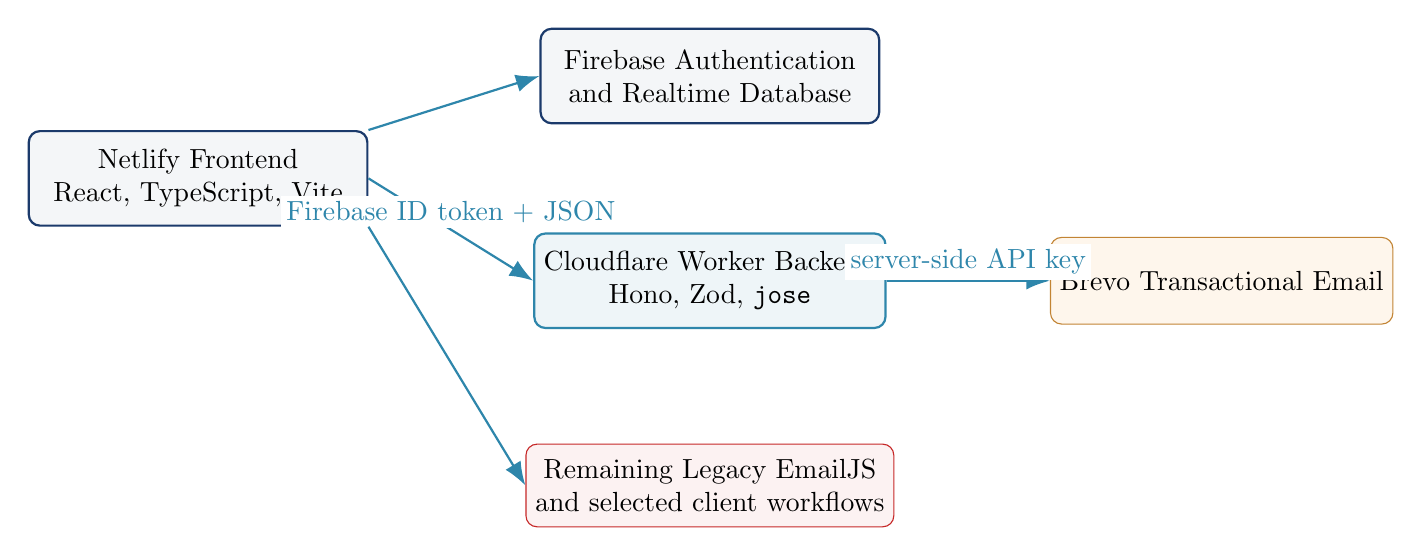
\begin{tikzpicture}[
  box/.style={draw=primary, rounded corners, fill=lightgray, minimum width=4.3cm, minimum height=1.2cm, align=center, thick},
  backend/.style={draw=secondary, rounded corners, fill=secondary!8, minimum width=4.3cm, minimum height=1.2cm, align=center, thick},
  external/.style={draw=accent!80!black, rounded corners, fill=accent!10, minimum width=4.0cm, minimum height=1.1cm, align=center},
  legacy/.style={draw=warnred, rounded corners, fill=warnred!6, minimum width=4.0cm, minimum height=1.05cm, align=center},
  arrow/.style={-{Latex[length=3mm]}, thick, color=secondary}
]
  \node[box] (browser) at (0,1.4) {Netlify Frontend\\React, TypeScript, Vite};
  \node[box] (firebase) at (6.5,2.7) {Firebase Authentication\\and Realtime Database};
  \node[backend] (worker) at (6.5,0.1) {Cloudflare Worker Backend\\Hono, Zod, \texttt{jose}};
  \node[external] (brevo) at (13.0,0.1) {Brevo Transactional Email};
  \node[legacy] (emailjs) at (6.5,-2.5) {Remaining Legacy EmailJS\\and selected client workflows};

  \draw[arrow] (browser.north east) -- (firebase.west);
  \draw[arrow] (browser.east) -- node[above,fill=white,inner sep=2pt]{Firebase ID token + JSON} (worker.west);
  \draw[arrow] (worker.east) -- node[above,fill=white,inner sep=2pt]{server-side API key} (brevo.west);
  \draw[arrow] (browser.south east) -- (emailjs.west);
\end{tikzpicture}}
\caption{Current hybrid architecture after the first backend migration}
\end{figure}

The backend is located inside the same repository under \path{backend/}, but it has its own \texttt{package.json}, source tree, tests, configuration, and deployment command.


\section{Technology Inventory}

\begin{table}[H]
\centering
\rowcolors{2}{lightgray}{white}
\begin{tabularx}{\linewidth}{@{}l l X@{}}
\toprule
\rowcolor{primary}
\textcolor{white}{\textbf{Layer}} & \textcolor{white}{\textbf{Technology}} & \textcolor{white}{\textbf{Current Use}} \\
\midrule
Frontend & React 19, TypeScript, Vite & Page rendering, feature orchestration, Firebase client access, meeting forms, and typed calls to the invitation backend. \\
Frontend hosting & Netlify & Production frontend builds and deployment at \path{https://lincministry.com}; repository secret scanning is enabled. \\
UI & Tailwind-style utility classes, Motion, AnimatePresence, Lucide icons, IntersectionObserver & Responsive bilingual interfaces, hero animations, carousel interactions, and a scroll-triggered floating action dock with reduced-motion support. \\
Identity & Firebase Authentication & Existing Google and email/password sessions; the invitation client silently obtains the current Firebase ID token. \\
Database & Firebase Realtime Database & Main storage for assessments, meetings, requests, availability, NextGen, attendance, groups, and notes. \\
Backend & Cloudflare Workers, Hono, TypeScript & First production API slice for authenticated participant meeting invitations and Brevo test delivery. \\
Runtime validation & Zod & Strict meeting-invitation request validation, including recipients, date, time ordering, locale, location, and optional meeting URL. \\
Token verification & \texttt{jose} & Firebase ID-token signature, issuer, audience, subject, and time-claim verification in the Worker. \\
Backend deployment & Wrangler & Local Worker development and explicit production deployment using \texttt{npx wrangler deploy}. \\
Email & Brevo and EmailJS & Participant meeting invitations use backend Brevo delivery; cancellation, People Development, and other legacy flows may still use EmailJS. \\
Testing & Vitest, Cloudflare Vitest pool & Worker-compatible route tests with mocked outbound Brevo requests. \\
Continuous integration & GitHub Actions & Backend tests run on relevant pushes and pull requests; deployment is not currently automated. \\
Storage & Base64 in Realtime Database; bucket configured & PDFs are embedded in database records; Firebase Storage is configured but not consistently used. \\
Legacy integrations & Gmail API, Google Calendar, OpenRouter & Referenced but not operationally required and selected for removal. \\
Configuration & YAML, environment variables, Wrangler variables, Worker secrets & Assessment definitions, public Firebase identifiers, local \texttt{.dev.vars}, and protected Brevo credentials. \\
Localization & Custom React context and flat dictionary & English/Arabic locale switching with significant inline-string duplication; backend invitation templates support English and Arabic. \\
\bottomrule
\end{tabularx}
\caption{Current technology inventory after the backend foundation}
\end{table}


\section{Current Authentication and Authorization}

The frontend continues to use Firebase Authentication and the existing \path{admins/} database branch for staff access decisions. Client components still interpret role labels and determine access to most current workflows.

The new participant meeting-invitation endpoint adds a narrower backend authentication boundary. The frontend obtains the current Firebase ID token from the already signed-in user and sends it through:

\begin{lstlisting}
Authorization: Bearer <firebase-id-token>
\end{lstlisting}

The Worker verifies the token using Google's Firebase signing keys and the \texttt{churchmeeting} project audience and issuer. Invalid, expired, or missing tokens are rejected with \texttt{401}. This reuses the existing Firebase session and does not introduce another login interface.

The implemented backend route currently proves authentication, not complete pastor-role authorization. An attempted backend Realtime Database role lookup was intentionally removed because it expanded the migration into an unrequested role-system redesign. The existing frontend pastor-access model remains unchanged for this slice. The long-term target remains backend-enforced capabilities for all sensitive actions.

\begin{warningbox}[-- Current Authorization Boundary]
A valid Firebase account can satisfy the current invitation endpoint's authentication check. The route does not yet prove the caller's Pastor capability. This is an accepted transitional boundary for the implemented slice, not the final enterprise authorization model. Anonymous access is blocked, but role enforcement, token-revocation checks, and rate limiting remain future controls.
\end{warningbox}


\section{Current Code Organization}

The codebase uses broad \texttt{components/} and \texttt{pages/} folders. Several files act as entire subsystems rather than focused UI components. The largest example is the calendar component, which combines scheduling, meeting requests, People Development, NextGen review, survey aggregation, file handling, personal notes, AI actions, and email templates.

The current organization leads to:

\begin{itemize}
  \item Duplicated business rules between pages and components.
  \item Coupling between UI state, database paths, notifications, and access logic.
  \item Difficult unit testing and migration.
  \item Large blast radius for small changes.
  \item Inconsistent models and pervasive \texttt{any} usage.
\end{itemize}

% ============================================================

% ============================================================
\chapter{Implemented Backend Foundation and Brevo Meeting Invitations}
% ============================================================

\section{Implementation Status}

This chapter documents completed implementation work rather than a future-state recommendation. The backend foundation, test route, Firebase token verification, participant meeting-invitation route, frontend client, automated tests, GitHub Actions workflow, CORS configuration, Netlify adjustment, and Cloudflare deployment were implemented during the July 24, 2026 backend work.

\begin{notebox}[-- Completed Production Slice]
The migrated participant meeting-invitation path now follows \texttt{React frontend $\rightarrow$ authenticated Cloudflare Worker $\rightarrow$ Brevo}. The Brevo API key is no longer required in browser code for this workflow.
\end{notebox}

\section{Scope and Migration Decision}

The backend work was intentionally incremental. It did not attempt to rewrite the entire Firebase application, replace the database, or redesign every permission. The selected first workflow was participant meeting invitations created from the Pastor Dashboard's Add Event form.

The previous sensitive path was conceptually:

\begin{center}
\texttt{Pastor Dashboard $\rightarrow$ browser EmailJS/provider call}
\end{center}

The implemented path is:

\begin{center}
\texttt{Pastor Dashboard $\rightarrow$ frontend API client $\rightarrow$ Cloudflare Worker $\rightarrow$ Brevo}
\end{center}

Meeting creation and the existing Firebase data model remain in place. Only the sensitive external email-provider call was moved behind the backend for this feature.

\section{Repository and File Hierarchy}

The backend was created in the existing repository under \path{backend/}. The implemented hierarchy is:

\begin{lstlisting}
backend/
|-- src/
|   |-- auth/
|   |   `-- firebaseAuth.ts
|   |-- emails/
|   |   `-- meetingInvitation.email.ts
|   |-- middleware/
|   |   `-- authentication.middleware.ts
|   |-- routes/
|   |   `-- meetingInvitations.routes.ts
|   |-- schemas/
|   |   `-- meetingInvitation.schema.ts
|   |-- services/
|   |   `-- brevo.service.ts
|   `-- index.ts
|-- test/
|   `-- index.spec.ts
|-- .dev.vars
|-- .gitignore
|-- package.json
|-- vitest.config.ts
`-- wrangler.jsonc
\end{lstlisting}

The frontend additions and modified integration point are:

\begin{lstlisting}
src/
|-- services/
|   `-- meetingInvitations.ts
`-- components/
    `-- pastor/
        `-- hooks/
            `-- useMeetings.ts
\end{lstlisting}

The GitHub Actions workflow is stored at:

\begin{lstlisting}
.github/workflows/backend-tests.yml
\end{lstlisting}

\section{Backend Initialization}

The backend was scaffolded using the Hono Cloudflare Workers template. The initial root route returned:

\begin{lstlisting}
Hello Hono!
\end{lstlisting}

This route remains a basic health check. The backend package contains its own dependencies and scripts, allowing frontend and backend development to remain separated even though they share one repository.

The principal backend dependencies are:

\begin{itemize}
  \item \textbf{Hono} for routing, middleware, JSON responses, and CORS.
  \item \textbf{Zod} for runtime validation.
  \item \textbf{\texttt{jose}} for Firebase JWT verification.
  \item \textbf{Wrangler} for Worker development and deployment.
  \item \textbf{Vitest} and \textbf{\texttt{@cloudflare/vitest-pool-workers}} for testing.
\end{itemize}

\section{Configuration and Secret Management}

The backend distinguishes public configuration from secret provider credentials.

\begin{table}[H]
\centering
\rowcolors{2}{lightgray}{white}
\begin{tabularx}{\linewidth}{@{}l l X@{}}
\toprule
\rowcolor{primary}
\textcolor{white}{\textbf{Binding}} & \textcolor{white}{\textbf{Classification}} & \textcolor{white}{\textbf{Purpose}} \\
\midrule
\texttt{FIREBASE\_PROJECT\_ID} & Public configuration & Firebase token audience and issuer validation; current value is \texttt{churchmeeting}. \\
\texttt{FIREBASE\_DATABASE\_URL} & Public configuration & Current Realtime Database identifier; retained for future backend use although no role lookup is used in the invitation route. \\
\texttt{BREVO\_API\_KEY} & Secret & Authorizes the Worker to call Brevo. \\
\texttt{BREVO\_SENDER\_EMAIL} & Protected configuration & Current verified sender address used by the Worker. \\
\texttt{BREVO\_SENDER\_NAME} & Protected configuration & Display name for outgoing mail. \\
\texttt{BREVO\_TEST\_RECIPIENT} & Protected configuration & Fixed recipient for the temporary backend test endpoint. \\
\bottomrule
\end{tabularx}
\caption{Implemented Worker configuration}
\end{table}

Local development values are stored in:

\begin{lstlisting}
backend/.dev.vars
\end{lstlisting}

The file is ignored by Git, and the ignore behavior was explicitly verified. Production provider values are configured as Cloudflare Worker secrets rather than committed to \texttt{wrangler.jsonc}.

The current non-secret Worker variables in \texttt{wrangler.jsonc} include:

\begin{lstlisting}
"vars": {
  "FIREBASE_PROJECT_ID": "churchmeeting",
  "FIREBASE_DATABASE_URL":
    "https://churchmeeting-default-rtdb.firebaseio.com"
}
\end{lstlisting}

\section{Brevo Test Endpoint}

A temporary test endpoint was implemented before the real application workflow:

\begin{lstlisting}
POST /api/v1/email/test
\end{lstlisting}

The request accepts a strict \texttt{sandbox} Boolean. In sandbox mode, the Worker sends the Brevo header:

\begin{lstlisting}
X-Sib-Sandbox: drop
\end{lstlisting}

This allows provider validation without delivery. The endpoint uses a fixed server-side recipient and therefore does not accept an arbitrary browser-provided address.

The endpoint was validated locally with a real email and after deployment with a production sandbox request.

\section{CORS Configuration}

The Worker applies CORS middleware to \path{/api/*}. The allowed origins are:

\begin{lstlisting}
https://lincministry.com
http://localhost:5173
\end{lstlisting}

The allowed request headers are:

\begin{lstlisting}
Content-Type
Authorization
\end{lstlisting}

The allowed methods are:

\begin{lstlisting}
GET
POST
OPTIONS
\end{lstlisting}

The preflight cache duration is 86,400 seconds. Production preflight behavior was verified before the invitation route was connected.

\section{Firebase ID-Token Verification}

The file \path{backend/src/auth/firebaseAuth.ts} uses \texttt{createRemoteJWKSet} and \texttt{jwtVerify} from \texttt{jose}. Verification is restricted to \texttt{RS256}. The expected audience is the Firebase project ID, and the expected issuer is:

\begin{lstlisting}
https://securetoken.google.com/churchmeeting
\end{lstlisting}

The verification module validates the token signature and standard time constraints, verifies issued-at and authentication-time claims, validates the subject length, and returns a normalized authenticated user containing:

\begin{lstlisting}
uid
email
emailVerified
name
picture
signInProvider
\end{lstlisting}

The middleware at \path{backend/src/middleware/authentication.middleware.ts} requires the Bearer header, verifies the token once, and stores both the user and token in the Hono request context.

The existing Firebase session is reused. The browser does not ask the Pastor to sign in a second time. Firebase can refresh the ID token through the existing authenticated session when required.

\section{Authorization Scope Correction}

During implementation, a backend middleware was initially created to query \path{admins/} and require the exact \texttt{pastor} value. This introduced a wider role-authorization redesign that was outside the intended migration scope. The role lookup was rejected and removed from the invitation route.

A subsequent suggestion to remove all token-authentication files was also corrected because it would have made the Brevo endpoint anonymously callable.

The accepted implementation is:

\begin{itemize}
  \item Require a valid Firebase-authenticated account.
  \item Reuse the existing frontend session.
  \item Do not introduce another login.
  \item Do not perform a new backend Pastor-role lookup in this slice.
  \item Preserve the current frontend Pastor-access model.
\end{itemize}

\section{Meeting Invitation Request Schema}

The Zod schema at \path{backend/src/schemas/meetingInvitation.schema.ts} accepts:

\begin{lstlisting}
{
  "locale": "en",
  "recipients": [
    {
      "email": "member@example.com",
      "name": "Member Name"
    }
  ],
  "meeting": {
    "title": "Meeting title",
    "date": "2026-07-30",
    "startTime": "10:00",
    "endTime": "11:00",
    "location": "LINC Ministry",
    "meetLink": ""
  }
}
\end{lstlisting}

Validation includes:

\begin{itemize}
  \item Locale restricted to English or Arabic.
  \item At least one recipient and a bounded recipient count.
  \item Valid recipient email syntax and field lengths.
  \item Strict \texttt{YYYY-MM-DD} calendar-date validation.
  \item Strict 24-hour \texttt{HH:mm} time validation.
  \item Meeting end time after start time.
  \item Required title and bounded location.
  \item Empty meeting link or a valid URL.
  \item Rejection of unknown object fields through strict schemas.
\end{itemize}

\section{Bilingual Email Builder}

The pure builder at \path{backend/src/emails/meetingInvitation.email.ts} creates English or Arabic invitation content. It generates both HTML and plain text.

The builder:

\begin{itemize}
  \item Formats dates and times with \texttt{Intl.DateTimeFormat}.
  \item Uses right-to-left HTML layout for Arabic.
  \item Includes title, date, time, location, recipient name, and optional link.
  \item Escapes user-controlled values before placing them into HTML.
  \item Applies a fallback location when no location is supplied.
  \item Does not call Firebase, Hono, Brevo, React, or another external service.
\end{itemize}

Keeping this function pure makes the email content independently testable.

\section{Reusable Brevo Provider Service}

The file \path{backend/src/services/brevo.service.ts} owns direct communication with:

\begin{lstlisting}
https://api.brevo.com/v3/smtp/email
\end{lstlisting}

It accepts recipient data and prepared email content, injects the Worker-side sender and API key, parses the provider response, extracts the message ID, and throws a structured \texttt{BrevoRequestError} when delivery fails.

The meeting route does not contain the low-level provider implementation, and the provider service does not contain meeting-domain rules.

\section{Meeting Invitation API}

The production route is:

\begin{lstlisting}
POST /api/v1/meeting-invitations
\end{lstlisting}

The route execution order is:

\begin{enumerate}
  \item Verify the Firebase ID token.
  \item Parse the JSON request.
  \item Validate the payload with Zod.
  \item Build one localized email per valid recipient.
  \item Send each invitation through the Brevo service.
  \item Collect successful and failed results.
  \item Return a structured result.
\end{enumerate}

\begin{table}[H]
\centering
\rowcolors{2}{lightgray}{white}
\begin{tabularx}{\linewidth}{@{}l X@{}}
\toprule
\rowcolor{primary}
\textcolor{white}{\textbf{Status}} & \textcolor{white}{\textbf{Meaning}} \\
\midrule
\texttt{201} & All requested invitations were delivered successfully. \\
\texttt{207} & Some invitations were delivered and some failed. \\
\texttt{400} & Invalid JSON or schema validation failure. \\
\texttt{401} & Missing, invalid, or expired Firebase authentication token. \\
\texttt{502} & No invitation could be delivered or the provider rejected the requests. \\
\bottomrule
\end{tabularx}
\caption{Implemented invitation API responses}
\end{table}

The browser provides structured meeting data, not arbitrary HTML. The backend controls the actual email template.

\section{Frontend API Client}

The frontend service at \path{src/services/meetingInvitations.ts} performs the following actions:

\begin{enumerate}
  \item Read \texttt{auth.currentUser}.
  \item Obtain the current Firebase ID token.
  \item Call the Worker endpoint.
  \item Send the token in the Bearer header.
  \item Send structured invitation JSON.
  \item Parse the backend response.
  \item Return a Boolean success result to the meeting hook.
\end{enumerate}

The default backend base URL is:

\begin{lstlisting}
https://linc-backend.linc-ministry.workers.dev
\end{lstlisting}

A \texttt{VITE\_BACKEND\_BASE\_URL} override may be used for another environment.

\section{Pastor Dashboard Integration}

The meeting hook at \path{src/components/pastor/hooks/useMeetings.ts} was updated so participant invitations call:

\begin{lstlisting}
sendMeetingInvitationsViaBackend(...)
\end{lstlisting}

The hook filters selected participants to usable email addresses and sends one batch request containing the current locale, recipient names, recipient emails, and meeting details.

The Add Event form in \path{PastorDashboard.tsx} submits through the current \texttt{useMeetings} hook. The hook barrel file correctly exports the modified implementation. This confirmed that the Add Event workflow is connected to the backend client.

Other email workflows have not all been migrated. Requester cancellation and People Development notifications may still use EmailJS. Their continued imports do not mean that participant invitations still use EmailJS.

\section{Automated Tests}

The Worker test configuration uses Vitest with the Cloudflare Worker test pool. The initial test suite proves:

\begin{enumerate}
  \item The root route returns \texttt{Hello Hono!}.
  \item Invalid sandbox input returns \texttt{400 VALIDATION\_ERROR}.
  \item A mocked successful Brevo sandbox request returns success without contacting the real provider.
\end{enumerate}

The tests passed locally after the invitation route was mounted.

Additional route-specific tests remain recommended for missing authentication, invalid tokens, invitation validation, complete success, partial failure, and complete provider failure.

\section{GitHub Actions}

The workflow at \path{.github/workflows/backend-tests.yml} runs for relevant backend pushes and pull requests. It uses Ubuntu, Node.js 24, \texttt{npm ci}, and \texttt{npm test} with the backend directory as the working directory.

The workflow is associated with backend foundation issue \#12. It verifies the backend but does not currently deploy the Worker.

\section{Netlify Secret-Scan Failure and Remediation}

The frontend TypeScript and Vite build succeeded, but Netlify failed the deployment during its secret-scanning stage. It detected the value of \texttt{VITE\_FIREBASE\_PROJECT\_ID} inside \path{backend/wrangler.jsonc}. The same public project identifier also appeared inside the Firebase database URL.

The value was not a private credential. Netlify was matching an environment-variable value against repository content.

The remediation was to add:

\begin{lstlisting}
SECRETS_SCAN_OMIT_KEYS=VITE_FIREBASE_PROJECT_ID
\end{lstlisting}

to the Netlify environment configuration. The variable itself was not marked as containing a secret. A new Netlify deployment was required after saving the setting.

\section{Separate Production Deployments}

The backend code was not activated by the Netlify redeployment. The Worker had to be deployed separately using:

\begin{lstlisting}
npx wrangler deploy
\end{lstlisting}

The apparent continued EmailJS behavior was therefore partly a deployment-version problem: the new frontend expected a route that had not yet been deployed to Cloudflare.

The operational rule is:

\begin{center}
\textbf{Frontend contract changes require Netlify deployment, and backend contract changes require Wrangler deployment.}
\end{center}

\section{Troubleshooting Lessons}

The production investigation established several lessons:

\begin{itemize}
  \item A successful Vite build does not prove a successful Netlify deployment.
  \item A Netlify secret-scan failure occurs after compilation and must be diagnosed separately.
  \item An EmailJS import warning does not prove that the tested runtime path invoked EmailJS.
  \item A remaining cancellation helper can keep EmailJS in a bundle even after participant invitations migrate.
  \item The actual call chain must be traced from the Add Event form to \texttt{useMeetings}, then to the frontend service, Worker route, and Brevo.
  \item The backend and frontend can be individually correct but incompatible when only one is deployed.
  \item The active production state must be verified at both hosting platforms.
\end{itemize}

\section{Current Security Improvements}

The implemented slice provides the following improvements:

\begin{itemize}
  \item The Brevo API key is absent from the React bundle.
  \item Anonymous callers are blocked by Firebase token verification.
  \item The backend validates all invitation data.
  \item The browser cannot provide arbitrary email HTML.
  \item Email HTML escapes meeting and recipient values.
  \item CORS is restricted to the production site and local frontend.
  \item Delivery failures are represented explicitly.
  \item Provider communication is centralized.
\end{itemize}

\section{Current Limitations}

The implemented slice intentionally does not yet provide:

\begin{itemize}
  \item Backend Pastor-role or capability enforcement.
  \item Firebase token-revocation checking.
  \item Cloudflare rate limiting.
  \item Queue-based retries or durable delivery jobs.
  \item A custom authenticated sender domain.
  \item Automatic Worker deployment from GitHub Actions.
  \item Migration of all EmailJS workflows.
  \item Audit records in the application database.
  \item Removal of the temporary Brevo test endpoint.
\end{itemize}

\section{Skills and Engineering Knowledge Developed}

The completed work developed and demonstrated the following practical skills:

\begin{enumerate}
  \item Incremental backend migration without rewriting the full application.
  \item Cloudflare Worker project creation, configuration, and deployment.
  \item Hono route composition, middleware, CORS, and JSON error design.
  \item Runtime validation using strict Zod schemas and business refinements.
  \item Separation of secret Worker bindings from public frontend configuration.
  \item Local secret management through \texttt{.dev.vars} and Git-ignore verification.
  \item Brevo transactional-email integration and sandbox testing.
  \item Firebase ID-token verification with remote JSON Web Keys.
  \item Reuse of an existing Firebase session without adding a second login flow.
  \item Bearer-token transport between a Vite frontend and a custom backend.
  \item Pure bilingual English/Arabic email-template construction.
  \item Right-to-left email rendering and localized date/time formatting.
  \item HTML escaping for user-controlled transactional-email values.
  \item Provider-adapter design and structured provider exceptions.
  \item Complete, partial, and failed multi-recipient delivery handling.
  \item Worker-compatible Vitest configuration and outbound request mocking.
  \item GitHub Actions continuous integration for a nested backend package.
  \item Netlify secret-scanner diagnosis and expected-value omission.
  \item Multi-platform production deployment management.
  \item Tracing a production event from UI submission to external provider.
  \item Distinguishing dependency-bundle warnings from runtime behavior.
  \item Correcting scope expansion when authentication work became an unrequested authorization overhaul.
  \item Balancing transitional security with preservation of the existing Pastor workflow.
  \item Documenting actual current architecture separately from target architecture.
\end{enumerate}

\section{Implemented Backend Details to Preserve}

The following details are authoritative for subsequent backend work:

\begin{itemize}
  \item Backend directory: \path{backend/}.
  \item Worker name: \texttt{linc-backend}.
  \item Worker URL: \path{https://linc-backend.linc-ministry.workers.dev}.
  \item Frontend URL: \path{https://lincministry.com}.
  \item Local frontend origin: \path{http://localhost:5173}.
  \item Firebase project ID: \texttt{churchmeeting}.
  \item Firebase database URL: \path{https://churchmeeting-default-rtdb.firebaseio.com}.
  \item Invitation endpoint: \path{/api/v1/meeting-invitations}.
  \item Temporary test endpoint: \path{/api/v1/email/test}.
  \item Frontend invitation client: \path{src/services/meetingInvitations.ts}.
  \item Frontend integration hook: \path{src/components/pastor/hooks/useMeetings.ts}.
  \item Participant meeting invitations use backend Brevo delivery.
  \item Existing Firebase authentication is reused silently.
  \item The current route requires authentication but not a backend Pastor-role lookup.
  \item CORS allows \texttt{Content-Type} and \texttt{Authorization}.
  \item Netlify omits \texttt{VITE\_FIREBASE\_PROJECT\_ID} from secret matching.
  \item GitHub Actions tests the backend but does not deploy it.
  \item Wrangler deployment remains a separate explicit action.
\end{itemize}


\chapter{Current Functional Modules}
% ============================================================

\section{Public Landing Page}

The landing page is active and visually mature, but it is hard-coded and positions the entire product as an assessment. It exposes six primary entry points: assessment, staff login, meeting booking, group notes, attendance, and NextGen activities. The page includes a presentation carousel using local placeholder shape tiles, but it does not yet include an administrator-managed carousel, Bible-verse manager, content publishing workflow, or Admin Mode.

A responsive floating action dock is now implemented. The original hero action area is observed using \texttt{IntersectionObserver}. Once that area has fully passed above the viewport, the same six actions are promoted into a fixed top navigation dock. When the user scrolls back until the original actions re-enter the viewport, the dock exits and the buttons resume their normal hero layout. The transition uses \texttt{AnimatePresence} and a spring animation, with an opacity-only fallback when the operating system requests reduced motion.

The floating dock is constrained to the viewport using full-width outer positioning, bounded horizontal padding, and a centered \texttt{max-w-5xl} container. On phones, actions use a two-column grid with wrapping text, a viewport-relative maximum height, and vertical overflow protection. On larger screens, the actions use a centered wrapping flex layout. The container applies backdrop blur, visible separation from page content, and pointer-event isolation so only the dock itself captures interaction.

\begin{infobox}[-- Implemented Interaction Contract]
The dock appears only after the original action group has moved above the viewport; it must not cover or replace the original buttons while they are visible. All six routes remain available in both layouts, English and Arabic directionality is preserved, the dock never exceeds the screen width, and scrolling back to the hero restores the original presentation without a page reload.
\end{infobox}

The current implementation duplicates some action-button markup between the hero and floating layouts. During component extraction, route, icon, label, and style metadata should be centralized in a shared action definition so the two presentations cannot drift.

\textbf{Disposition:} retain the visual foundation and floating action-dock behavior, broaden product identity, extract landing sections and shared action definitions, and connect published content to a secured content-management API.

\section{Assessment Engine}

The assessment engine is a valuable generic YAML-driven component. It supports fields, grouped ratings, rating lists, scoring strategies, ranking, and bilingual results. It stores a common record with metadata, fields, scores, and bilingual result objects.

The same component also contains direct signup and member-linkage administration. A browser-side passcode protects some linkage operations, which is not an acceptable security boundary. Email logic and identifier management are also embedded in the component.

\textbf{Disposition:} retain and isolate the YAML engine; move submission validation, persistence, identity linkage, and notifications to backend services.

\section{Assessment Definitions}

Two reviewed YAML definitions provide active assessment content:

\begin{itemize}
  \item Five Service Pathways.
  \item Spiritual Gifts Discovery.
\end{itemize}

The YAML files contain executable configuration and descriptive metadata. Some fields are not implemented by the renderer, including declared email providers, detailed validation rules, report formats, and selected metadata. The same assessment text is partly duplicated in the static translation dictionary.

\textbf{Disposition:} make YAML the authoritative source for assessment-specific content, validate definitions during CI, version definitions, and remove unused declarative fields or implement them consistently.

\section{Public Meeting Booking}

The active public booking page reads availability, confirmed meetings, unavailability, and administrator accounts directly from Firebase. It creates pending requests and sends emails to all administrator emails. A duplicate \texttt{BookMeeting} component contains similar logic and additionally blocks pending requests.

\textbf{Disposition:} retain one public booking interface; delete the duplicate; publish only sanitized availability; claim slots atomically through the backend; notify only configured Pastor recipients.

\section{Pastor Calendar and Operations}

The calendar component is the central operational monolith. It manages meetings, availability, unavailability, meeting requests, participant data, People Development assignments, PDFs, personal notes, NextGen approvals, questions, survey results, and AI calendar actions.

\textbf{Disposition:} continue the decomposition into separate feature modules and backend services. Participant meeting invitations have already moved to the Cloudflare Worker and Brevo. Delete remaining AI mutation paths, Google integration, fake Meet links, browser-exposed model credentials, and legacy EmailJS workflows in later slices.

\section{NextGen Activities}

The NextGen subsystem is functionally rich. It supports registration, Pastor approval, four-character identifiers, question submission, voting, survey responses, participation history, and certificate generation. Firebase transactions correctly protect uniqueness and one-vote/one-response constraints in several flows.

The primary risk is that a short identifier is treated as authentication. Survey responses described as anonymous are linked to identifiers and personal information.

\textbf{Disposition:} retain the domain workflows; use authenticated accounts or secure invitation tokens; keep the short ID as a public reference only; clarify or redesign survey anonymity.

\section{Attendance}

Attendance includes person creation and editing, Sunday recording, and analysis. Access is protected by a predictable passcode formula embedded in the browser. Attendance is stored as a comma-separated list of dates inside person records.

\textbf{Disposition:} replace passcode access with authenticated capabilities; normalize attendance into sessions and records; add corrections, audit, deactivation, duplicate handling, and historical analysis rules.

\section{People Development and Group Notes}

The congregation group portal uses a participant identifier to locate member and form records, then downloads all assignments and filters them in the browser. Group PDFs are stored as base64 data in Realtime Database.

\textbf{Disposition:} use authenticated member identity, group-scoped API responses, object storage, signed download URLs, and canonical group definitions.

\section{Pastoral Notes}

The pastoral notes page stores people, strengths, growth areas, follow-up dates, and comments. The page reads all notes before checking whether the user is allowed to edit. Records use email addresses as author identity and can be permanently deleted without an audit trail.

\textbf{Disposition:} classify as highly confidential, enforce Pastor-only backend access, use immutable audit events, implement soft deletion and version history, and deny General Admin access by default.

\section{Localization}

The custom i18n provider is sound for English and Arabic, but translation coverage is inconsistent. Stable UI strings are split between a flat dictionary and inline bilingual conditions. Assessment content is duplicated between translations and YAML.

\textbf{Disposition:} retain the provider, type translation keys, split namespaces, centralize stable UI strings, and keep administrator-created bilingual content in database records.

\section{Legal and Guide Pages}

The Guide, Privacy Policy, and Terms are active pages with outdated content. They still describe Google/Gmail workflows and an assessment-only application. They do not disclose the full data categories handled by NextGen, attendance, groups, or pastoral notes.

\textbf{Disposition:} retain page shells; rewrite content after the architecture, providers, retention rules, and access controls are finalized.

% ============================================================
\chapter{Current Data Model and Data Flows}
% ============================================================

\section{Observed Realtime Database Paths}

\begin{longtable}{@{}p{0.30\linewidth} p{0.28\linewidth} p{0.34\linewidth}@{}}
\toprule
\rowcolor{primary}
\textcolor{white}{\textbf{Path}} & \textcolor{white}{\textbf{Purpose}} & \textcolor{white}{\textbf{Primary Concern}} \\
\midrule
\endfirsthead
\toprule
\rowcolor{primary}
\textcolor{white}{\textbf{Path}} & \textcolor{white}{\textbf{Purpose}} & \textcolor{white}{\textbf{Primary Concern}} \\
\midrule
\endhead
\path{form/} & Assessment submissions and direct-signup records & Mixed record types, compatibility aliases, broad reads, and identity duplication. \\
\path{meetings/} & Confirmed Pastor meetings & Public clients may receive confidential details. \\
\path{meetingRequests/} & Pending, accepted, and rejected requests & Race conditions, personal reasons, and duplicated workflow logic. \\
\path{availability/} & Pastor booking availability & Direct writes and hard-coded booking policy. \\
\path{unavailability/} & Schedule blocks & Public exposure of reasons and schedule details. \\
\path{admins/} & Email-keyed role records & Obsolete superadmin model, client authorization, and notification overreach. \\
\path{nextGenUsers/} & Registration and approval records & Four-character identifiers used as authentication. \\
\path{nextGenActivities/qaSessions/} & Questions and voting & Identity-linked votes and client-side migrations. \\
\path{nextGenActivities/participationByIdentifier/} & Participation history & Identifier-based access and fragmented person identity. \\
\path{nextGenActivities/surveys/.../responsesByIdentifier/} & Survey responses & Described as anonymous but identity is retained. \\
\path{attendance/people/} & People and date lists & Denormalized dates, weak access control, and duplicate-person risk. \\
\path{peopleDevelopment/members/} & Member profiles & Overlaps with forms, attendance, NextGen, and notes. \\
\path{peopleDevelopment/assignments/} & Group files and notes & Full assignment reads, base64 files, and group filtering in browser. \\
\path{peopleDevelopment/personalNotes/} & Strength/weakness notes & Sensitive data mixed into operational subsystem. \\
\path{peopleNotes/} & Pastoral care records & Highly confidential, broad reads, no versioned audit. \\
\bottomrule
\caption{Observed Firebase path inventory}
\end{longtable}

\section{Identity Fragmentation}

A single human may appear separately in:

\begin{itemize}
  \item Assessment submissions.
  \item People Development members.
  \item Attendance people.
  \item NextGen users.
  \item Pastoral notes.
  \item Meeting requests.
\end{itemize}

Different aliases, identifiers, emails, and record keys are used to connect these records. This fragmentation causes duplicate people, inconsistent updates, difficult deletion requests, unclear access boundaries, and complex reporting.

\begin{decisionbox}[-- Canonical Member Identity]
The target architecture shall introduce a canonical \texttt{Member} entity. Feature records reference a stable member identifier where identity is known. Anonymous or external submissions may exist temporarily, but must be linkable through controlled reconciliation rather than repeated compatibility scans.
\end{decisionbox}

\section{Current Sensitive Data Flows}

The current browser often receives more data than it needs. Examples include:

\begin{itemize}
  \item Public booking clients reading meeting and unavailability records.
  \item Group-note clients reading complete member, form, and assignment collections before filtering.
  \item Pastoral-note clients reading all notes before UI checks.
  \item Attendance logic storing and analyzing full person history in the browser.
  \item Email workflows receiving recipient lists and message content in frontend code.
\end{itemize}

The target system must apply data minimization at the API boundary. A client receives only fields required for the specific operation.

% ============================================================
\chapter{Current-State Risk Assessment}
% ============================================================

\section{Risk Rating Method}

Risks are rated using qualitative likelihood and impact. Priority is derived from the combination of confidentiality, integrity, availability, legal exposure, and operational consequences.

\begin{longtable}{@{}p{0.07\linewidth} p{0.25\linewidth} p{0.12\linewidth} p{0.12\linewidth} p{0.12\linewidth} p{0.22\linewidth}@{}}
\toprule
\rowcolor{primary}
\textcolor{white}{\textbf{ID}} & \textcolor{white}{\textbf{Risk}} & \textcolor{white}{\textbf{Likelihood}} & \textcolor{white}{\textbf{Impact}} & \textcolor{white}{\textbf{Priority}} & \textcolor{white}{\textbf{Required Treatment}} \\
\midrule
\endfirsthead
\toprule
\rowcolor{primary}
\textcolor{white}{\textbf{ID}} & \textcolor{white}{\textbf{Risk}} & \textcolor{white}{\textbf{Likelihood}} & \textcolor{white}{\textbf{Impact}} & \textcolor{white}{\textbf{Priority}} & \textcolor{white}{\textbf{Required Treatment}} \\
\midrule
\endhead
R-01 & Direct browser access to confidential database branches & High & Critical & Critical & Introduce backend API; deny direct client reads and writes. \\
R-02 & UI role checks mistaken for authorization & High & Critical & Critical & Backend capability enforcement and restrictive database rules. \\
R-03 & Short identifiers and predictable passcodes used as authentication & High & High & Critical & Firebase Auth, invitations, verified sessions, and capability checks. \\
R-04 & Browser-exposed AI/OpenRouter credentials and mutation capabilities & High & Critical & Critical & Remove AI mutation functions and rotate any exposed credentials. \\
R-05 & Public exposure of meeting names, reasons, and schedules & Medium & High & High & Publish sanitized availability only. \\
R-06 & Race conditions in meeting booking and multi-step workflows & High & High & High & Database transactions, idempotency keys, and backend orchestration. \\
R-07 & General administrator receiving Pastor notifications or data & Medium & High & High & Capability-scoped recipients and separation of duties. \\
R-08 & Highly confidential pastoral notes lack audit and versioning & Medium & Critical & Critical & Pastor-only service, immutable audit events, and soft delete. \\
R-09 & Base64 files stored in Realtime Database & High & Medium & High & Object storage, malware controls, metadata, signed URLs, and quotas. \\
R-10 & Survey described as anonymous while identity is stored & High & High & High & Redesign anonymity or update claims and access controls. \\
R-11 & Legal policies do not match actual data practices & High & High & High & Rewrite after service and data-flow finalization. \\
R-12 & Duplicate person records across modules & High & Medium & High & Canonical member model and migration. \\
R-13 & Duplicate booking and business logic implementations & High & Medium & High & Delete duplicate component and centralize domain logic. \\
R-14 & Non-operational Google/Gmail and fake Meet features & High & Medium & Medium & Remove dependencies, UI, translations, and credentials. \\
R-15 & Missing audit, monitoring, and retry handling for email workflows & High & Medium & High & Notification service, delivery states, retries, and observability. \\
R-16 & Hard-coded role provisioning and service identifiers & Medium & Critical & Critical & Remove, rotate, and manage through secure configuration. \\
R-17 & No verified migration, backup, or rollback process & Medium & High & High & Formal migration runbooks, snapshots, checksums, and rollback tests. \\
R-18 & Large monolithic components and pervasive untyped data & High & Medium & High & Feature modules, schemas, domain types, and automated tests. \\
\bottomrule
\caption{Current-state risk register}
\end{longtable}

\section{Security Risks}

The highest security issue is architectural: the client is both user interface and application server. The browser contains data-access paths, provider identifiers, workflow decisions, notification content, and authorization assumptions. Even strong Firebase Rules cannot easily provide the orchestration, field-level filtering, logging, rate limiting, and cross-entity transactions required by the platform.

\section{Privacy Risks}

The system handles multiple categories of confidential information. Pastoral notes are especially sensitive. The current Privacy Policy does not describe all categories or external processors, and some interfaces retrieve entire collections before filtering. Data minimization, retention, deletion, and access review are not consistently defined.

\section{Integrity Risks}

Many operations combine several steps:

\begin{itemize}
  \item Write a request.
  \item Create or update a meeting.
  \item Send email.
  \item Update status.
  \item Write audit information.
\end{itemize}

When executed in the browser, partial failure can leave inconsistent records. Some errors are silently ignored. The backend must own state transitions and record each step.

\section{Maintainability Risks}

The codebase contains monolithic files, duplicated services, inconsistent type models, inline translations, compatibility parsing, and mixed responsibilities. These issues increase defect probability and make onboarding difficult. They also reduce commercial transfer value because the product depends on undocumented knowledge held by its original developer.

% ============================================================
\chapter{Pruning and Refactoring Decisions}
% ============================================================

\section{Components and Features to Remove}

\begin{longtable}{@{}p{0.30\linewidth} p{0.14\linewidth} p{0.47\linewidth}@{}}
\toprule
\rowcolor{primary}
\textcolor{white}{\textbf{Item}} & \textcolor{white}{\textbf{Status}} & \textcolor{white}{\textbf{Decision}} \\
\midrule
\endfirsthead
\toprule
\rowcolor{primary}
\textcolor{white}{\textbf{Item}} & \textcolor{white}{\textbf{Status}} & \textcolor{white}{\textbf{Decision}} \\
\midrule
\endhead
\texttt{AIBookingAssistant.tsx} & \statusremove & Delete entirely. It duplicates booking rules, exposes browser AI configuration, uses conflicting durations, and can report false success. \\
AI operations in the Pastor calendar & \statusremove & Remove natural-language database mutation and all exposed model credentials. \\
\texttt{BookMeeting.tsx} & \statusremove & Delete after final repository-wide call-site verification. Transfer only the concept that pending requests temporarily occupy slots. \\
Google OAuth callback flow & \statusremove & Remove because Google login/integration is not operationally required. \\
Gmail API sending & \statusremove & Remove and replace with a backend notification adapter. \\
Google Calendar event creation & \statusremove & Remove unless reintroduced later as a server-side, separately approved integration. \\
Fake Meet-link generator & \statusremove & Delete production placeholder behavior and related translations. \\
\texttt{superadmin} role & \statusremove & Remove from types, routes, checks, data, and documentation. \\
\texttt{AdminDashboard.tsx} & \statusremove & Delete obsolete wrapper page. Replace with a new Admin Mode workspace. \\
\texttt{AdminManager.tsx} & \statusremove & Delete browser-based role management and automatic provisioning. \\
Hard-coded default administrator emails & \statusremove & Remove immediately and rotate any associated credentials. \\
Unused Firestore initialization & \statusverify & Remove if a complete repository search confirms no use. \\
Legacy translation keys & \statusremove & Remove alongside deleted Google, AI, superadmin, and duplicate booking code. \\
Base64 PDF persistence & \statusremove & Stop creating new base64 file records; migrate existing files to object storage. \\
\bottomrule
\caption{Confirmed pruning decisions}
\end{longtable}

\section{Modules to Retain and Modernize}

\begin{table}[H]
\centering
\rowcolors{2}{lightgray}{white}
\begin{tabularx}{\linewidth}{@{}l l X@{}}
\toprule
\rowcolor{primary}
\textcolor{white}{\textbf{Module}} & \textcolor{white}{\textbf{Status}} & \textcolor{white}{\textbf{Modernization Direction}} \\
\midrule
Landing page & \statusrefactor & Preserve the implemented floating action dock, rebrand as portal, extract sections and shared action definitions, and add managed content, carousel, verses, and feature flags. \\
Assessment engine & \statusrefactor & Keep YAML renderer; move validation, submission, linking, and email to backend. \\
Booking calendar & \statusrefactor & Keep one interface; consume sanitized API; use atomic backend reservations. \\
Pastor calendar & \statusrefactor & Split into focused modules and services. \\
NextGen & \statusrefactor & Keep workflows; replace identifier authentication and clarify anonymity. \\
Attendance & \statusrefactor & Replace passcode and normalize sessions/records. \\
Group portal & \statusrefactor & Authenticate members, return scoped assignments, use object storage. \\
Pastoral notes & \statusrefactor & Pastor-only confidential service with audit and retention controls. \\
I18n provider & \statusactive & Keep; add typed keys, namespaces, fallbacks, and centralized strings. \\
Page title and layout & \statusrefactor & Make workspace-aware and capability-driven. \\
Guide and legal pages & \statusrefactor & Rewrite content after architecture completion. \\
\bottomrule
\end{tabularx}
\caption{Retain-and-modernize decisions}
\end{table}

% ============================================================
\chapter{Target Enterprise Architecture}
% ============================================================

\section{Architecture Principles}

The target design follows these principles:

\begin{enumerate}
  \item \textbf{Backend authority:} all sensitive reads, writes, decisions, and transactions pass through the API.
  \item \textbf{Least privilege:} each user receives only the capabilities and fields required.
  \item \textbf{Separation of duties:} technical administration does not imply pastoral authority.
  \item \textbf{Canonical identity:} one member identity is referenced across features.
  \item \textbf{Transactional integrity:} state transitions are atomic and idempotent.
  \item \textbf{Privacy by design:} confidential data is minimized, classified, retained, and audited.
  \item \textbf{Modularity:} frontend, backend, and domain models are organized by feature boundaries.
  \item \textbf{Observability:} important actions produce logs, metrics, delivery states, and audit events.
  \item \textbf{Progressive migration:} the system can move to the target architecture without a high-risk rewrite cutover.
\end{enumerate}

\section{Recommended Target Stack}

A pragmatic target stack is:

\begin{itemize}
  \item \textbf{Frontend:} React, TypeScript, Vite, feature modules, typed API client.
  \item \textbf{Backend:} Cloudflare Workers with Hono and TypeScript are the implemented foundation. The platform may continue with structured Hono feature modules or move selected workloads to NestJS or another managed TypeScript service when background jobs, relational transactions, or runtime requirements exceed the edge-worker model.
  \item \textbf{Authentication:} Firebase Authentication retained initially; ID tokens verified by the backend through Firebase Admin SDK.
  \item \textbf{Primary database:} PostgreSQL for transactional and relational domain data.
  \item \textbf{Migration bridge:} Firebase Realtime Database retained temporarily behind backend repositories during staged migration.
  \item \textbf{File storage:} Firebase Storage or Google Cloud Storage with metadata in the primary database.
  \item \textbf{Notifications:} provider-agnostic backend adapters. Brevo is already implemented for participant meeting invitations; remaining EmailJS flows should migrate incrementally.
  \item \textbf{Deployment:} Netlify for the current static frontend and Cloudflare Workers for the implemented edge backend. Managed containers or job runtimes may be added for workloads that require longer execution, queues, or private database connectivity.
  \item \textbf{Observability:} structured logs, exception tracking, metrics, health checks, and audit-event storage.
\end{itemize}

\begin{decisionbox}[-- Progressive Database Strategy]
Do not require an immediate all-at-once database rewrite. First introduce the backend as an API facade over the current Firebase data. Once direct client access is disabled and workflows are centralized, migrate high-value domains to PostgreSQL in controlled phases. This delivers security and orchestration benefits early while reducing cutover risk.
\end{decisionbox}

\section{Target Architecture Diagram}

\begin{figure}[H]
\centering
\resizebox{0.90\textwidth}{!}{%
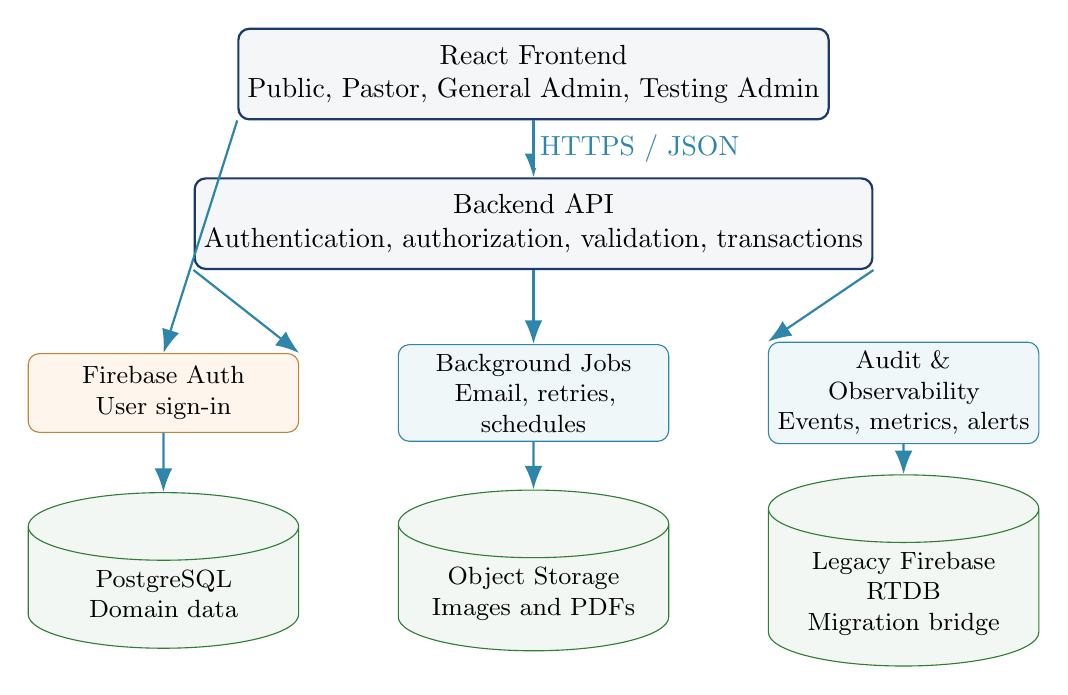
\begin{tikzpicture}[
  box/.style={draw=primary, rounded corners, fill=lightgray, minimum width=5.2cm, minimum height=1.15cm, align=center, thick},
  service/.style={draw=secondary, rounded corners, fill=secondary!7, text width=3.2cm, minimum height=1.0cm, align=center, font=\small},
  data/.style={draw=notegreen, cylinder, shape border rotate=90, aspect=0.25, fill=notegreen!6, text width=3.2cm, minimum height=1.3cm, align=center, font=\small},
  external/.style={draw=accent!80!black, rounded corners, fill=accent!10, text width=3.2cm, minimum height=1.0cm, align=center, font=\small},
  arrow/.style={-{Latex[length=3mm]}, thick, color=secondary}
]
  \node[box] (frontend) at (0,4.25) {React Frontend\\Public, Pastor, General Admin, Testing Admin};
  \node[box] (api) at (0,2.35) {Backend API\\Authentication, authorization, validation, transactions};

  \node[external] (auth) at (-4.7,0.20) {Firebase Auth\\User sign-in};
  \node[service] (jobs) at (0,0.20) {Background Jobs\\Email, retries, schedules};
  \node[service] (audit) at (4.7,0.20) {Audit \&\\Observability\\Events, metrics, alerts};

  \node[data] (postgres) at (-4.7,-2.35) {PostgreSQL\\Domain data};
  \node[data] (storage) at (0,-2.35) {Object Storage\\Images and PDFs};
  \node[data] (legacydb) at (4.7,-2.35) {Legacy Firebase\\RTDB\\Migration bridge};

  \draw[arrow] (frontend) -- node[right,fill=white,inner sep=2pt]{HTTPS / JSON} (api);
  \draw[arrow] (frontend.south west) -- (auth.north);
  \draw[arrow] (api.south west) -- (auth.north east);
  \draw[arrow] (api) -- (jobs);
  \draw[arrow] (api.south east) -- (audit.north west);
  \draw[arrow] (auth) -- (postgres);
  \draw[arrow] (jobs) -- (storage);
  \draw[arrow] (audit) -- (legacydb);
\end{tikzpicture}}
\caption{Target three-tier architecture with backend authority, protected data stores, jobs, and audit controls}
\end{figure}

\section{Frontend Responsibilities}

The frontend shall:

\begin{itemize}
  \item Render public and authenticated interfaces.
  \item Manage local interaction state and optimistic presentation where safe.
  \item Obtain Firebase ID tokens and call the backend API.
  \item Display only data returned by authorized endpoints.
  \item Perform convenience validation while treating backend validation as authoritative.
  \item Use typed request and response models generated from an API contract where practical.
  \item Avoid embedding service secrets, database paths, privileged recipient lists, or workflow decisions.
  \item Preserve context-aware navigation behaviors such as the landing-page floating action dock without allowing fixed elements to exceed the viewport or obscure critical content.
  \item Respect \texttt{prefers-reduced-motion}, keyboard navigation, focus visibility, RTL direction, and screen-reader labels for animated navigation.
  \item Centralize action metadata so normal and floating presentations share routes, icons, labels, and capability or feature-flag rules.
\end{itemize}

\section{Backend Responsibilities}

The backend shall own:

\begin{multicols}{2}
\begin{itemize}
  \item Authentication-token verification.
  \item Capability authorization.
  \item Request validation and schema parsing.
  \item Booking conflict transactions.
  \item Pastor decisions and state transitions.
  \item NextGen registration, voting, and survey integrity.
  \item Attendance session writes and corrections.
  \item Member reconciliation.
  \item File metadata and signed access.
  \item Notification rendering and delivery.
  \item Audit events.
  \item Rate limiting and abuse controls.
  \item Reporting and aggregation.
  \item Data retention and deletion workflows.
  \item Migration adapters.
\end{itemize}
\end{multicols}

\section{Database Responsibilities}

The primary database shall enforce unique constraints, foreign keys, transactions, and normalized domain relationships. Sensitive application tables must never be directly accessible from the browser. Database access shall be limited to backend identities and migration tooling.

% ============================================================
\chapter{Authorization and Administration Methodology}
% ============================================================

\section{Role Model}

The target role model separates ministry authority from technical administration.

\begin{table}[H]
\centering
\rowcolors{2}{lightgray}{white}
\begin{tabularx}{\linewidth}{@{}l X X@{}}
\toprule
\rowcolor{primary}
\textcolor{white}{\textbf{Role}} & \textcolor{white}{\textbf{Purpose}} & \textcolor{white}{\textbf{Explicit Boundary}} \\
\midrule
Pastor & Perform pastoral decisions, manage schedule, review participants, approve NextGen activity, and access pastoral notes. & Does not automatically manage technical configuration or administrator authorities. \\
General Admin & Manage Admin Mode, public content, feature flags, approved operational configuration, and delegated administrator permissions. & Cannot make ordinary Pastor decisions or access confidential pastoral notes by default. \\
Testing Admin & Validate UI, content drafts, feature configuration, and staging workflows. & No production Pastor decisions; production sensitive data is masked or unavailable by default. \\
Attendance Operator & Record and correct attendance and manage permitted attendance people. & No Pastor decisions, pastoral notes, or general administration unless separately granted. \\
Technical Maintainer & Deploy, monitor, migrate, and support the platform. & Privileged access is exceptional, audited, time-bounded where possible, and not used for routine ministry decisions. \\
\bottomrule
\end{tabularx}
\caption{Target role model}
\end{table}

\section{Capability Model}

Roles are convenience bundles. Authorization is enforced using capabilities. Example capability namespaces include:

\begin{lstlisting}[language=TypeScript,caption={Illustrative capability catalog}]
type Capability =
  | 'pastor.workspace.view'
  | 'booking.availability.manage'
  | 'booking.requests.view'
  | 'booking.requests.decide'
  | 'nextgen.registrations.review'
  | 'nextgen.questions.moderate'
  | 'peopleDevelopment.assignments.manage'
  | 'pastoralNotes.view'
  | 'pastoralNotes.create'
  | 'pastoralNotes.update'
  | 'attendance.view'
  | 'attendance.record'
  | 'attendance.people.manage'
  | 'adminMode.access'
  | 'carousel.manage'
  | 'carousel.publish'
  | 'bibleVerses.manage'
  | 'features.manage'
  | 'admins.manage'
  | 'pastor.preview';
\end{lstlisting}

\section{Non-Delegable Pastor Authority}

General Administrators may assign administrative capability bundles within a defined policy, but they must not grant themselves or others Pastor decision capabilities through ordinary Admin Mode. Pastor authority should require a separately controlled assignment process, such as approval by designated ministry leadership or a protected system-maintainer workflow.

\section{Pastor Preview}

A General Admin may need to see the Pastor interface to validate layouts and configuration. This shall be implemented as a read-only preview mode using masked, synthetic, or explicitly approved data. Preview mode must display a persistent banner and must not expose decision buttons or production confidential records.

\section{Admin Mode}

Admin Mode will provide structured management for:

\begin{itemize}
  \item Landing-page content.
  \item Carousel slides and image uploads.
  \item Bible verses.
  \item Public feature flags.
  \item Navigation visibility.
  \item Content ordering and scheduling.
  \item Draft, preview, publish, and rollback.
  \item Administrator authorities within policy.
  \item Audit history.
\end{itemize}

Each content item shall support bilingual fields, status, author, timestamps, order, effective dates, and version history.

% ============================================================
\chapter{Target Domain Model}
% ============================================================

\section{Core Entities}

\begin{longtable}{@{}p{0.24\linewidth} p{0.30\linewidth} p{0.38\linewidth}@{}}
\toprule
\rowcolor{primary}
\textcolor{white}{\textbf{Entity}} & \textcolor{white}{\textbf{Purpose}} & \textcolor{white}{\textbf{Key Relationships}} \\
\midrule
\endfirsthead
\toprule
\rowcolor{primary}
\textcolor{white}{\textbf{Entity}} & \textcolor{white}{\textbf{Purpose}} & \textcolor{white}{\textbf{Key Relationships}} \\
\midrule
\endhead
UserAccount & Authenticated system identity & Optional link to Member; many roles and capabilities. \\
Member & Canonical person record & Assessments, attendance, groups, NextGen, meetings, and pastoral records. \\
Role & Named capability bundle & Assigned to UserAccount through scoped assignments. \\
Capability & Atomic authorization unit & Included in roles and evaluated by backend policies. \\
AssessmentDefinition & Versioned YAML-derived assessment schema & Many submissions; immutable after publication. \\
AssessmentSubmission & Participant responses and results & Definition version and optional Member. \\
MeetingRequest & Requested date, slot, reason, requester, and status & May produce one Meeting after Pastor decision. \\
Meeting & Confirmed calendar event & Request, Pastor, participants, notifications. \\
AvailabilityWindow & Bookable Pastor time range & Used by slot computation and reservations. \\
SlotReservation & Temporary or confirmed booking claim & Unique by Pastor/date/start time. \\
NextGenRegistration & Registration and approval status & Member and participation records. \\
NextGenQuestion & Submitted question and moderation state & Votes and session. \\
Vote & One member vote for one question & Unique constraint on member and question. \\
SurveyDefinition & Versioned survey structure & Survey responses. \\
SurveyResponse & Participant answers & Anonymous token or confidential member link, never ambiguously both. \\
AttendanceSession & A service/event attendance date & Many AttendanceRecords. \\
AttendanceRecord & Member attendance status & Unique member/session pair with recorder identity. \\
PeopleGroup & Ministry or development group & Members, assignments, files, and notes. \\
GroupAssignment & Published group-specific content & Files, notes, effective dates, and audience. \\
PastoralNote & Highly confidential observation & Member, Pastor author, versions, follow-ups. \\
ContentItem & Versioned public or internal content & Carousel, verse, feature, or page section subtype. \\
FileObject & Stored-file metadata & Owner entity, storage key, checksum, MIME type, and access policy. \\
Notification & Delivery request and state & Template, recipient, provider, retries, and related domain event. \\
AuditEvent & Immutable record of sensitive activity & Actor, action, resource, timestamp, and context. \\
\bottomrule
\caption{Target domain entities}
\end{longtable}

\section{Canonical Member Model}

The canonical member record should contain stable identity and contact fields, while sensitive feature-specific data remains in separate tables. Suggested fields include:

\begin{lstlisting}[language=TypeScript,caption={Conceptual member model}]
interface Member {
  id: string;
  status: 'active' | 'inactive' | 'merged';
  fullName: string;
  preferredName?: string;
  primaryEmail?: string;
  primaryPhone?: string;
  locale?: 'en' | 'ar';
  createdAt: string;
  updatedAt: string;
  mergedIntoMemberId?: string;
}
\end{lstlisting}

Pastoral notes, assessment answers, attendance history, and group assignments are not embedded in the member row. This limits accidental over-fetching and supports separate retention and authorization policies.

\section{Content Model}

Public content shall use a versioned publication model:

\begin{itemize}
  \item \texttt{draft}: editable and visible only to authorized previews.
  \item \texttt{scheduled}: approved for future publication.
  \item \texttt{published}: active for public users.
  \item \texttt{archived}: retained for history but not displayed.
\end{itemize}

Carousel images and group documents are stored in object storage. Database records contain metadata and access rules, not raw base64 content.

% ============================================================
\chapter{API Design}
% ============================================================

\section{API Standards}

The backend API shall use:

\begin{itemize}
  \item Versioned endpoints such as \path{/api/v1}.
  \item Firebase ID-token authentication initially.
  \item JSON request and response bodies.
  \item Schema validation for every write.
  \item Consistent error envelopes and machine-readable codes.
  \item Idempotency keys for booking, notification, and other retryable writes.
  \item Pagination for collections.
  \item Server-generated timestamps.
  \item Correlation IDs for logging and support.
\end{itemize}

\section{Illustrative Endpoint Catalog}

\begin{longtable}{@{}p{0.12\linewidth} p{0.35\linewidth} p{0.43\linewidth}@{}}
\toprule
\rowcolor{primary}
\textcolor{white}{\textbf{Method}} & \textcolor{white}{\textbf{Endpoint}} & \textcolor{white}{\textbf{Purpose}} \\
\midrule
\endfirsthead
\toprule
\rowcolor{primary}
\textcolor{white}{\textbf{Method}} & \textcolor{white}{\textbf{Endpoint}} & \textcolor{white}{\textbf{Purpose}} \\
\midrule
\endhead
GET & \path{/api/v1/public/config} & Return published feature flags, navigation, and safe public settings. \\
GET & \path{/api/v1/public/landing} & Return published landing sections, carousel, and Bible verses. \\
GET & \path{/api/v1/public/booking/slots} & Return sanitized available/held/booked states without private details. \\
POST & \path{/api/v1/public/booking/requests} & Atomically reserve a slot and create a meeting request. \\
GET & \path{/api/v1/pastor/meeting-requests} & List authorized request details. \\
POST & \path{/api/v1/pastor/meeting-requests/{id}/accept} & Accept request, create meeting, and queue notifications. \\
POST & \path{/api/v1/pastor/meeting-requests/{id}/reject} & Reject request and queue configured notification. \\
GET & \path{/api/v1/assessments/definitions} & Return active assessment definitions. \\
POST & \path{/api/v1/assessments/{definitionId}/submissions} & Validate, score, persist, and queue result notification. \\
POST & \path{/api/v1/nextgen/registrations} & Create secure registration and public reference ID. \\
POST & \path{/api/v1/nextgen/questions/{id}/votes} & Record one authorized vote transactionally. \\
POST & \path{/api/v1/attendance/sessions/{id}/records} & Create or correct an attendance record with audit. \\
GET & \path{/api/v1/groups/me/assignments} & Return assignments scoped to authenticated member groups. \\
GET & \path{/api/v1/pastoral-notes} & Pastor-only, filtered and paginated notes. \\
POST & \path{/api/v1/admin/content/carousel} & Create a draft carousel item. \\
POST & \path{/api/v1/admin/content/{id}/publish} & Publish an approved content version. \\
GET & \path{/api/v1/admin/audit-events} & Return authorized audit history. \\
\bottomrule
\caption{Illustrative target endpoints}
\end{longtable}

\section{Error Envelope}

\begin{lstlisting}[caption={Standard API error response}]
{
  "error": {
    "code": "BOOKING_SLOT_UNAVAILABLE",
    "message": "The selected slot is no longer available.",
    "correlationId": "req_01J...",
    "details": {
      "date": "2026-08-15",
      "startTime": "14:30"
    }
  }
}
\end{lstlisting}

\section{API Documentation}

The backend shall publish an OpenAPI specification. The frontend client and integration tests should use generated types where practical. Each endpoint must document authentication, required capabilities, data classification, rate limits, request schema, response schema, error codes, and audit behavior.

% ============================================================
\chapter{Critical Workflow Specifications}
% ============================================================

\section{Meeting Booking}

The booking workflow shall prevent double booking and hide private schedule information.

\begin{enumerate}
  \item The client requests sanitized availability for a date range.
  \item The backend calculates candidate slots from availability, unavailability, confirmed meetings, and active reservations.
  \item The client submits one selected slot with requester information and an idempotency key.
  \item The backend starts a transaction and creates a unique slot reservation.
  \item If the slot is already held or booked, the transaction fails with a conflict response.
  \item A pending meeting request is created and linked to the reservation.
  \item Notification jobs are queued for configured Pastor recipients.
  \item Acceptance converts the reservation to booked and creates a meeting atomically.
  \item Rejection releases the reservation according to policy.
\end{enumerate}

\begin{criticalbox}[-- Booking Privacy]
The public endpoint must never return requester names, meeting titles, unavailability reasons, private notes, or Pastor contact lists. Public consumers receive slot state only.
\end{criticalbox}

\section{Assessment Submission}

The backend loads the published definition version, validates all required fields and rating ranges, calculates scores using a deterministic engine, stores the immutable definition version and result, and queues notification. Email failure does not invalidate a successful submission; delivery status is recorded separately.

\section{NextGen Voting}

Voting requires an authenticated or securely invited participant. A database unique constraint enforces one vote per participant per question. Aggregate counts may be returned publicly or to authorized participants, while individual voter identity is restricted.

\section{Attendance Recording}

Attendance is recorded against a defined session. The backend enforces a unique member/session record and records who created or corrected it. Corrections create audit history rather than silently replacing the record.

\section{Pastoral Decisions}

Pastoral actions such as meeting acceptance, NextGen approval, group assignment, and pastoral-note access require explicit Pastor capabilities. General Admin preview mode cannot invoke these endpoints, even if the interface is visible.

\section{Content Publishing}

Admin content follows draft, review, publish, and rollback stages. Every publish action records the actor, previous version, new version, effective time, and change summary. Public endpoints return only published content.

% ============================================================
\chapter{Security and Privacy Architecture}
% ============================================================

\section{Security Objectives}

The target system shall protect confidentiality, integrity, availability, accountability, and privacy. Security controls are applied at identity, API, database, storage, deployment, and operational layers.

\section{Authentication}

Firebase Authentication may be retained to reduce migration risk. The frontend obtains an ID token, and the backend verifies token signature, issuer, audience, expiry, revocation status where required, and user status. Authentication alone never implies authorization.

Public submissions shall use rate limiting, abuse detection, validation, and optional verification appropriate to the risk. Sensitive participant portals require authenticated or securely invited sessions rather than shared identifiers.

\section{Authorization}

Every sensitive endpoint declares required capabilities. Authorization is evaluated in the backend using current role assignments and policy rules. Database queries are scoped by the authorized principal and requested resource. The frontend does not decide access.

\section{Secrets Management}

No privileged API key, service account, email credential, recipient list, or database administrative secret may be embedded in the frontend bundle. Secrets shall be stored in a managed secret service and exposed only to backend runtime identities.

All previously browser-exposed or hard-coded secrets must be rotated during Phase 0.

\section{Data Classification}

\begin{table}[H]
\centering
\rowcolors{2}{lightgray}{white}
\begin{tabularx}{\linewidth}{@{}l X X@{}}
\toprule
\rowcolor{primary}
\textcolor{white}{\textbf{Class}} & \textcolor{white}{\textbf{Examples}} & \textcolor{white}{\textbf{Minimum Controls}} \\
\midrule
Public & Published landing content, verses, feature availability & Integrity control, versioning, and public read only. \\
Internal & Non-sensitive configuration and operational metadata & Authenticated access and audit for changes. \\
Confidential & Assessments, attendance, group membership, meeting requests & Capability authorization, minimization, encryption in transit, audit, retention. \\
Highly confidential & Pastoral notes, growth observations, care comments & Pastor-only access, strict audit, no broad exports, soft delete, access review. \\
Restricted technical & Secrets, service accounts, migration credentials & Secret manager, least privilege, rotation, no client exposure. \\
\bottomrule
\end{tabularx}
\caption{Target data classification}
\end{table}

\section{Audit Logging}

Audit events shall be immutable and include:

\begin{itemize}
  \item Actor user ID and effective role/capability context.
  \item Action and resource type.
  \item Resource identifier.
  \item Timestamp and correlation ID.
  \item Result: success, denial, or failure.
  \item Relevant before/after metadata without unnecessarily copying sensitive text.
  \item Administrative mode or preview context.
\end{itemize}

\section{Notification Security}

Notification templates and recipient selection are controlled by the backend. Delivery is asynchronous. Each notification records state such as queued, sent, failed, retrying, or cancelled. Sensitive content is minimized, and provider errors are observable rather than silently ignored.

\section{Privacy Governance}

The platform shall define retention periods by data category, a deletion and correction process, legal-policy versioning, and access-review procedures. Surveys must be explicitly anonymous or explicitly confidential; ambiguous claims are prohibited.

% ============================================================
\chapter{Data Migration Strategy}
% ============================================================

\section{Migration Objectives}

The migration must improve architecture without losing participant history or interrupting ministry operations. It shall be reversible at each major stage and produce reconciliation evidence.

\section{Migration Phases}

\begin{enumerate}
  \item \textbf{Inventory and backup:} export all Firebase branches, files, rules, and account metadata; calculate counts and checksums.
  \item \textbf{Backend facade:} introduce API endpoints that continue using Firebase through backend repositories.
  \item \textbf{Client cutover:} migrate frontend features to the API and disable corresponding direct Firebase operations.
  \item \textbf{Canonical identity:} create members and controlled reconciliation mappings.
  \item \textbf{Domain migration:} move booking, attendance, NextGen, groups, and pastoral records into PostgreSQL in priority order.
  \item \textbf{File migration:} decode base64 documents, upload to object storage, validate checksums, and replace database payloads with metadata references.
  \item \textbf{Rule lockdown:} deny client access to migrated branches and retain read-only legacy data only as required.
  \item \textbf{Decommission:} remove compatibility code and archive final exports after retention approval.
\end{enumerate}

\section{Path-to-Domain Mapping}

\begin{longtable}{@{}p{0.30\linewidth} p{0.30\linewidth} p{0.31\linewidth}@{}}
\toprule
\rowcolor{primary}
\textcolor{white}{\textbf{Current Path}} & \textcolor{white}{\textbf{Target Domain}} & \textcolor{white}{\textbf{Migration Note}} \\
\midrule
\endfirsthead
\toprule
\rowcolor{primary}
\textcolor{white}{\textbf{Current Path}} & \textcolor{white}{\textbf{Target Domain}} & \textcolor{white}{\textbf{Migration Note}} \\
\midrule
\endhead
\path{form/} & AssessmentSubmission / RegistrationImport & Discriminate by form ID and submission mode; preserve original payload as source metadata. \\
\path{meetings/} & Meeting & Link to Pastor, requester/member, and source request where possible. \\
\path{meetingRequests/} & MeetingRequest / SlotReservation & Normalize status transitions and detect duplicate slots. \\
\path{availability/} & AvailabilityWindow & Normalize dates, time zones, owner, and recurrence if introduced. \\
\path{unavailability/} & ScheduleBlock & Separate public slot effect from private reason. \\
\path{nextGenUsers/} & NextGenRegistration & Replace short ID authentication with account or invitation link. \\
\path{nextGenActivities/...} & Question, Vote, SurveyResponse & Preserve counts and identify legacy migration records. \\
\path{attendance/people/} & Member, AttendanceSession, AttendanceRecord & Split comma-separated dates into normalized rows. \\
\path{peopleDevelopment/members/} & Member / MemberProfile & Reconcile against assessments, attendance, and NextGen. \\
\path{peopleDevelopment/assignments/} & PeopleGroup / GroupAssignment / FileObject & Upload documents to storage and preserve display order. \\
\path{peopleNotes/} & PastoralNote / PastoralNoteVersion & Apply highly confidential classification and author mapping. \\
\path{admins/} & UserAccount / RoleAssignment & Translate Pastor accounts; do not migrate superadmin semantics. \\
\bottomrule
\caption{Current-to-target migration mapping}
\end{longtable}

\section{Migration Verification}

Each migration must produce:

\begin{itemize}
  \item Source record count.
  \item Target record count.
  \item Rejected and quarantined records.
  \item Identity merge decisions.
  \item File checksum results.
  \item Sample business-level validation.
  \item Rollback instructions.
  \item Approval evidence.
\end{itemize}

% ============================================================
\chapter{Frontend Modernization}
% ============================================================

\section{Target Repository Structure}

\begin{lstlisting}[caption={Recommended frontend organization}]
src/
  app/
    router/
    providers/
    authorization/
    configuration/
  features/
    assessments/
      components/
      api/
      models/
      definitions/
    booking/
    pastor-calendar/
    nextgen/
    attendance/
    people-development/
    pastoral-notes/
    admin-mode/
  shared/
    components/
    i18n/
    api/
    validation/
    utilities/
  pages/
\end{lstlisting}

\section{Typed API Client}

All server interactions should use a shared client that adds authentication tokens, correlation IDs, error parsing, and request cancellation. Domain features should not import Firebase database functions directly.

\section{State and Data Fetching}

Use a consistent query/cache approach for server state. Local component state remains appropriate for form inputs and presentation. Sensitive data should not be cached longer than required. Mutation success should be based on confirmed server responses, not stale React state.

\section{Localization}

The i18n provider shall use exact typed keys. Stable UI text is organized by feature namespace. Assessment-specific questions remain in versioned YAML definitions. Administrator-created content uses bilingual data fields with publication validation.

\section{Accessibility}

The modernization shall include:

\begin{itemize}
  \item Keyboard navigation and visible focus.
  \item Direction-aware icons and layout.
  \item Reduced-motion support.
  \item Accessible labels and error messages.
  \item Color contrast validation.
  \item Screen-reader announcements for async status.
  \item Accessible calendar and modal behavior.
  \item Scroll-triggered navigation that remains reachable by keyboard, does not trap focus, and does not cover the viewport on small screens.
  \item Motion fallbacks that replace spring travel with a short opacity transition when reduced motion is requested.
\end{itemize}

\section{Navigation and Workspaces}

The current \texttt{isAdmin}/\texttt{isSuperAdmin} layout props are replaced by authorization context. Desktop and mobile navigation show only authorized and enabled destinations. Mode indicators clearly identify Pastor, Admin, Testing, Attendance, and Preview contexts.

% ============================================================
\chapter{Backend Implementation Design}
% ============================================================

\section{Implemented Foundation Versus Target Modules}

The current Worker is intentionally smaller than the final module map. It already separates authentication, middleware, schemas, routes, email builders, and provider services. This is the correct starting discipline. Future domains should extend these boundaries rather than moving all application behavior into \path{backend/src/index.ts}.

\section{Recommended Module Boundaries}

\begin{lstlisting}[caption={Recommended backend modules}]
src/
  auth/
  authorization/
  users/
  members/
  assessments/
  booking/
  meetings/
  nextgen/
  attendance/
  people-development/
  pastoral-notes/
  content/
  files/
  notifications/
  audit/
  reporting/
  migrations/
  common/
\end{lstlisting}

\section{Layering}

Each feature should contain:

\begin{itemize}
  \item Controller or transport layer.
  \item Application service or use-case layer.
  \item Domain models and policies.
  \item Repository interfaces.
  \item Infrastructure adapters for PostgreSQL, Firebase, storage, and email.
  \item Unit and integration tests.
\end{itemize}

Controllers should not contain domain decisions. Repositories should not render email. Notification providers should not update booking state. These boundaries prevent a new backend monolith from replacing the current frontend monolith.

\section{Validation}

Use runtime schemas for every input, migration record, and external provider response. Validation rules belong near the domain model and are shared through generated contracts or duplicated intentionally with backend authority.

\section{Transactions and Idempotency}

Transactional workflows include booking, vote creation, survey response creation, attendance correction, member merging, content publication, and Pastor decisions. Idempotency keys prevent duplicate writes when clients retry after network failure.

\section{Background Jobs}

Email, scheduled publication, expired booking holds, data exports, migration batches, and periodic reports should run through background jobs rather than browser loops. Failed jobs are retried with bounded policies and dead-letter handling.

% ============================================================
\chapter{Testing and Quality Strategy}
% ============================================================

\section{Testing Pyramid}

\begin{table}[H]
\centering
\rowcolors{2}{lightgray}{white}
\begin{tabularx}{\linewidth}{@{}l X X@{}}
\toprule
\rowcolor{primary}
\textcolor{white}{\textbf{Test Level}} & \textcolor{white}{\textbf{Coverage}} & \textcolor{white}{\textbf{Examples}} \\
\midrule
Unit & Pure domain rules and utilities & Assessment scoring, slot overlap, capability policy, survey anonymity, date calculations. \\
Service & Application use cases with repositories mocked & Accept meeting request, record attendance, publish content, merge members. \\
Integration & Real database and provider adapters in test environment & Unique constraints, transactions, migrations, signed file URLs, notification state. \\
Contract & API request/response compatibility & OpenAPI schema, frontend client generation, error codes. \\
End-to-end & User journeys across frontend and backend & Assessment submission, booking, Pastor approval, NextGen vote, attendance correction. \\
Security & Authorization and abuse cases & Privilege escalation, IDOR, rate limits, token expiry, cross-group access. \\
Accessibility & Keyboard and assistive technology behavior & Calendars, forms, modals, alerts, RTL navigation, floating action dock, reduced-motion behavior. \\
Performance & Load and response-time behavior & Public slots, assessment submission, reporting, file access. \\
Migration & Historical data correctness & Counts, checksums, identity merges, rollback. \\
\bottomrule
\end{tabularx}
\caption{Target quality strategy}
\end{table}

\section{Critical Automated Tests}

The initial critical suite shall prove:

\begin{itemize}
  \item General Admin cannot invoke Pastor decisions.
  \item Testing Admin cannot alter production data.
  \item Public users cannot read meeting identities or pastoral data.
  \item Two simultaneous booking requests cannot reserve the same slot.
  \item One participant cannot vote twice for the same question.
  \item Attendance correction records an audit event.
  \item Pastoral notes are unavailable without the required capabilities.
  \item Deleted or disabled features are inaccessible by direct URL and API.
  \item Email failure does not corrupt domain state.
  \item Published content is immutable except through new versions.
  \item The floating action dock appears only after the original hero actions pass above the viewport and disappears when they return.
  \item Every floating action remains inside the viewport and usable at narrow mobile widths in both English and Arabic.
  \item Reduced-motion mode avoids spring translation while preserving the dock state change and navigation access.
\end{itemize}

\section{Definition of Done}

A feature is not complete until it has:

\begin{itemize}
  \item Documented requirements and acceptance criteria.
  \item Backend authorization and validation.
  \item Database migration where required.
  \item Unit, integration, and relevant end-to-end tests.
  \item Bilingual interface coverage.
  \item Audit and observability behavior.
  \item Updated API and user documentation.
  \item Security and privacy review.
\end{itemize}

% ============================================================
\chapter{DevOps, Deployment, and Operations}
% ============================================================

\section{Current Implemented Delivery Pipeline}

The current production system has three operational automation surfaces:

\begin{itemize}
  \item \textbf{Netlify} builds and publishes the React frontend.
  \item \textbf{Cloudflare Wrangler} deploys the Worker backend manually.
  \item \textbf{GitHub Actions} runs backend tests for relevant pushes and pull requests.
\end{itemize}

The frontend build runs \texttt{tsc -b \&\& vite build}. Netlify additionally performs repository secret scanning. The backend test workflow runs \texttt{npm ci} and \texttt{npm test} from the \path{backend/} directory. Automated Worker deployment is not yet configured.

\begin{warningbox}[-- Deployment Coupling]
An API change is not complete in production until the compatible frontend and Worker versions are both deployed. Release notes and future CI/CD should treat the two artifacts as one coordinated release even when hosted independently.
\end{warningbox}

\section{Environments}

The platform shall maintain separate environments:

\begin{itemize}
  \item \textbf{Local development:} local services or emulators with synthetic data.
  \item \textbf{Testing/staging:} representative infrastructure, masked or synthetic data, and Testing Admin access.
  \item \textbf{Production:} restricted deployment, audited access, and production service identities.
\end{itemize}

Production data must not be copied into test environments without an approved anonymization process.

\section{CI/CD Pipeline}

The pipeline shall include:

\begin{enumerate}
  \item Dependency installation with lockfile enforcement.
  \item Formatting and linting.
  \item Type checking.
  \item Unit and integration tests.
  \item Assessment-definition validation.
  \item Security and secret scanning.
  \item Backend and frontend builds.
  \item Database migration validation.
  \item Staging deployment and smoke tests.
  \item Approved production promotion.
  \item Post-deployment health verification.
\end{enumerate}

\section{Configuration and Secrets}

Environment configuration is validated at startup. Secrets reside in a managed secret store and are injected into backend runtime only. Frontend environment variables are treated as public and may contain only non-secret configuration.

\section{Monitoring}

Minimum operational telemetry includes:

\begin{itemize}
  \item API request volume, latency, and errors.
  \item Authentication and authorization denials.
  \item Booking conflicts and reservation expiry.
  \item Notification delivery and retries.
  \item Background-job failures.
  \item Database connection and migration status.
  \item File upload and access errors.
  \item Security alerts and unusual access patterns.
\end{itemize}

\section{Backup and Recovery}

PostgreSQL and object storage require automated backups, tested restore procedures, retention policies, and documented recovery objectives. Firebase exports remain part of migration and historical recovery until decommissioning is approved.

\section{Incident Response}

The runbook shall define severity, triage, containment, communication, evidence preservation, recovery, and post-incident review. Incidents involving pastoral records or participant data require privacy-impact assessment and leadership notification.

% ============================================================
\chapter{Documentation and Governance}
% ============================================================

\section{Required Documentation Set}

The final repository should include:

\begin{itemize}
  \item Root README with architecture, setup, and links.
  \item Local-development guide.
  \item Environment and secret reference.
  \item OpenAPI documentation.
  \item Database schema and migration guide.
  \item Authorization and capability catalog.
  \item Administrator and Pastor user guides.
  \item Testing strategy and commands.
  \item Deployment and rollback runbooks.
  \item Incident-response runbook.
  \item Data-retention and deletion procedures.
  \item Architecture Decision Records.
  \item Change log and release notes.
\end{itemize}

\section{Architecture Decision Records}

Key decisions shall be captured as ADRs, including:

\begin{itemize}
  \item Introduction of the backend tier.
  \item Choice of backend framework.
  \item PostgreSQL adoption and Firebase migration strategy.
  \item Capability-based authorization.
  \item Pastor and Admin separation of duties.
  \item Object-storage model.
  \item Survey anonymity policy.
  \item Notification provider.
  \item Legal-content versioning.
\end{itemize}

\section{Governance Reviews}

At least quarterly, review:

\begin{itemize}
  \item Role and capability assignments.
  \item Pastor access to highly confidential data.
  \item General Admin and Testing Admin boundaries.
  \item Stale accounts.
  \item Retention and deletion queues.
  \item Audit anomalies.
  \item Provider and dependency changes.
  \item Privacy and legal text accuracy.
\end{itemize}

% ============================================================
\chapter{Implementation Roadmap}
% ============================================================

\section{Phase 0: Immediate Risk Reduction}

\textbf{Objective:} eliminate exposed and misleading legacy paths before broader redesign.

\begin{taskbox}[-- Deliverables]
\begin{itemize}
  \item Remove AI booking and AI calendar mutations.
  \item Remove Google/Gmail/Calendar and fake Meet features.
  \item Remove hard-coded default administrators and superadmin flows.
  \item Rotate exposed or hard-coded credentials.
  \item Delete duplicate booking component after call-site verification.
  \item Snapshot Firebase data and Rules.
  \item Add temporary protective Rules and logging where feasible.
\end{itemize}
\end{taskbox}

\textbf{Indicative effort:} 60--120 hours.

\section{Phase 1: Backend Foundation}

\begin{itemize}
  \item Establish backend project, health checks, structured logging, and CI/CD.
  \item Verify Firebase ID tokens.
  \item Implement user, role, capability, and audit foundations.
  \item Add configuration validation and secret management.
  \item Create API facade repositories over Firebase.
\end{itemize}

\textbf{Indicative effort:} 180--280 hours.

\begin{notebox}[-- Phase 1 Partial Completion]
The initial Cloudflare Worker package, Hono entry point, Brevo provider adapter, Firebase token verification, CORS, Zod validation, Vitest tests, GitHub Actions testing, and one production frontend-to-backend workflow are complete. Capability authorization, audit persistence, rate limiting, broader repositories, automatic deployment, and additional domains remain outstanding.
\end{notebox}


\section{Phase 2: Booking and Notifications}

\begin{itemize}
  \item Create sanitized slot endpoint.
  \item Implement slot reservations and transactional requests.
  \item Move acceptance/rejection and meeting creation to backend.
  \item Centralize notification templates, recipients, retries, and delivery status.
  \item Cut public booking and Pastor calendar request flows over to API.
\end{itemize}

\textbf{Indicative effort:} 140--220 hours.

\section{Phase 3: Identity and Member Consolidation}

\begin{itemize}
  \item Define canonical member model.
  \item Build reconciliation tools and merge audit.
  \item Link assessment, attendance, NextGen, groups, and meetings.
  \item Remove browser-wide identity scans.
\end{itemize}

\textbf{Indicative effort:} 140--240 hours.

\section{Phase 4: Admin Mode and Public Content}

\begin{itemize}
  \item Create General Admin and Testing Admin workspaces.
  \item Implement capability delegation policy.
  \item Add carousel, Bible verses, landing sections, feature flags, and navigation controls.
  \item Extract the implemented floating action dock into a maintainable landing-navigation component with centralized action metadata and responsive regression tests.
  \item Add drafts, preview, publish, scheduling, version history, and rollback.
  \item Upload images through object storage.
\end{itemize}

\textbf{Indicative effort:} 180--300 hours.

\section{Phase 5: NextGen, Attendance, and Groups}

\begin{itemize}
  \item Replace identifier-based authentication.
  \item Move voting and survey rules into backend transactions.
  \item Normalize attendance sessions and records.
  \item Replace attendance passcode with authenticated capabilities.
  \item Scope group assignments and migrate PDFs to object storage.
\end{itemize}

\textbf{Indicative effort:} 220--360 hours.

\section{Phase 6: Pastoral Notes and High-Sensitivity Controls}

\begin{itemize}
  \item Implement Pastor-only note service.
  \item Add versioning, follow-up workflow, soft deletion, and audit.
  \item Implement preview masking and access reviews.
  \item Define retention and correction procedures.
\end{itemize}

\textbf{Indicative effort:} 100--180 hours.

\section{Phase 7: PostgreSQL Migration and Decommissioning}

\begin{itemize}
  \item Create relational schema and migrations.
  \item Move domains in controlled batches.
  \item Reconcile counts and historical records.
  \item Disable direct client Firebase access.
  \item Remove compatibility code and archive legacy exports.
\end{itemize}

\textbf{Indicative effort:} 180--320 hours.

\section{Phase 8: Enterprise Hardening and Commercial Readiness}

\begin{itemize}
  \item Complete security, accessibility, and load testing.
  \item Finalize privacy, Terms, and user guides.
  \item Add monitoring, backups, restore tests, and incident runbooks.
  \item Produce deployment packages, onboarding materials, and support procedures.
  \item Complete independent architecture and security review.
\end{itemize}

\textbf{Indicative effort:} 120--220 hours.

\section{Roadmap Summary}

\begin{table}[H]
\centering
\rowcolors{2}{lightgray}{white}
\begin{tabularx}{\linewidth}{@{}l l l X@{}}
\toprule
\rowcolor{primary}
\textcolor{white}{\textbf{Phase}} & \textcolor{white}{\textbf{Effort}} & \textcolor{white}{\textbf{Dependency}} & \textcolor{white}{\textbf{Primary Outcome}} \\
\midrule
0 & 60--120 h & None & Immediate risk reduction and legacy removal. \\
1 & 180--280 h & Phase 0 & Backend, authorization, audit, and API facade. \\
2 & 140--220 h & Phase 1 & Secure booking and notifications. \\
3 & 140--240 h & Phase 1 & Canonical member identity. \\
4 & 180--300 h & Phases 1 and 3 & Admin Mode and configurable public content. \\
5 & 220--360 h & Phases 1 and 3 & Secured NextGen, attendance, and groups. \\
6 & 100--180 h & Phases 1 and 3 & High-confidentiality pastoral notes. \\
7 & 180--320 h & Prior API cutovers & PostgreSQL migration and Firebase lockdown. \\
8 & 120--220 h & All core phases & Enterprise hardening and transfer readiness. \\
\bottomrule
\end{tabularx}
\caption{Modernization roadmap summary}
\end{table}

% ============================================================
\chapter{Acceptance Criteria and Enterprise Readiness}
% ============================================================

\section{Architecture Acceptance}

The modernization is architecturally complete when:

\begin{itemize}
  \item No confidential domain is read or written directly from the browser.
  \item Every sensitive operation is authorized by backend capability checks.
  \item The superadmin model and hard-coded provisioning are absent.
  \item General Admin and Pastor authority are technically separated.
  \item The frontend contains no privileged secrets or provider credentials.
  \item Transactional workflows use database transactions and idempotency.
\end{itemize}

\section{Security Acceptance}

\begin{itemize}
  \item Authorization tests prove denial across roles and resources.
  \item Public APIs return no private meeting, member, or pastoral fields.
  \item Short identifiers and attendance codes are not authentication factors.
  \item Secrets are rotated and stored in a managed secret service.
  \item Audit events exist for role changes, Pastor decisions, note access, attendance corrections, content publication, and data exports.
  \item Security review finds no critical or high unresolved issues.
\end{itemize}

\section{Data Acceptance}

\begin{itemize}
  \item Canonical member mapping is complete or all unresolved duplicates are quarantined.
  \item Migration counts and checksums reconcile.
  \item Base64 files are migrated and verified.
  \item Historical records remain accessible according to retention policy.
  \item Backup and restore tests succeed.
\end{itemize}

\section{Product Acceptance}

\begin{itemize}
  \item Public content is managed through drafts and publishing.
  \item Carousel and Bible verses support English and Arabic.
  \item The floating landing-page action dock preserves all six actions, stays within the viewport at supported widths, respects RTL and reduced-motion settings, and returns cleanly to the original hero layout.
  \item Disabled features are hidden and inaccessible.
  \item Pastor, General Admin, Testing Admin, and attendance experiences are clearly distinguished.
  \item Legal pages accurately describe retained data and services.
  \item End-to-end tests cover every critical user journey.
\end{itemize}

\section{Commercial Transfer Acceptance}

The product is commercially transferable when a competent engineering team can deploy, operate, support, and extend it without undocumented knowledge from the original developer. This requires complete setup instructions, API documentation, schema migrations, runbooks, test evidence, architecture decisions, licences, dependency inventory, and clear intellectual-property ownership.

% ============================================================
\chapter{Indicative Budget and Commercial Positioning}
% ============================================================

\section{Engineering Budget}

The roadmap represents approximately 1,150--1,930 hours. At a blended professional engineering rate of CAD 80 per hour, the indicative implementation budget is approximately CAD 92,000--154,400. This is an engineering planning estimate rather than a fixed quotation. Scope, staffing, infrastructure, security review, legal review, and migration complexity may change the total.

\section{Post-Modernization Asset Value}

A completed, documented, tested, and deployable system with no recurring revenue is primarily valued by replacement cost, transferability, and strategic fit. A reasonable target sale range after successful modernization is approximately CAD 80,000--120,000, with higher value possible when the transaction includes exclusive intellectual property, deployment support, onboarding, and maintenance.

Recurring revenue and demonstrated adoption can materially increase value because the product would then be assessed as an operating software business rather than only a code asset.

\section{Recommended Commercial Model}

The strongest long-term option is to retain the intellectual property and license deployments to multiple ministries, with implementation, hosting, support, and optional customization. An exclusive sale should be considered only when the offer reflects the value of the domain model, migration tooling, documentation, operational readiness, and future revenue opportunity.

% ============================================================
\chapter{Conclusion}
% ============================================================

The LINC Ministry Portal contains a meaningful set of ministry workflows and demonstrates strong product initiative. Its current weakness is not a lack of functionality; it is that most domains still lack a backend boundary, unified data model, enforceable authorization architecture, and operational discipline appropriate to the sensitivity of the data.

The completed Cloudflare Worker and Brevo meeting-invitation migration proves that the system can be modernized incrementally without disrupting the existing Pastor experience. The browser now acts as an authenticated client for this workflow, the Worker validates the request and protects the provider credential, and Brevo delivery is separated from React code. This is the first concrete implementation of the target three-tier direction.

The modernization must continue beyond reorganizing React files. Authority should progressively move into backend services. The database should become a protected persistence layer rather than a public application interface.

By removing legacy AI, Google, Gmail, superadmin, duplicate booking, and base64-storage code; introducing a three-tier architecture; consolidating identity; enforcing capabilities; and building separate Pastor, Admin, and Testing workspaces, the platform can become secure, maintainable, enterprise-grade, and commercially transferable.

\begin{infobox}[-- Final Direction]
The target is not a larger version of the current frontend. The implemented invitation Worker is the first backend slice, and the target is to extend that pattern into a properly engineered ministry platform with explicit domain boundaries, auditable authority, and a controlled migration path from the current hybrid system.
\end{infobox}

% ============================================================
\appendix
\chapter{Current File Classification Matrix}
% ============================================================

\begin{longtable}{@{}p{0.30\linewidth} p{0.14\linewidth} p{0.48\linewidth}@{}}
\toprule
\rowcolor{primary}
\textcolor{white}{\textbf{File / Area}} & \textcolor{white}{\textbf{Classification}} & \textcolor{white}{\textbf{Action}} \\
\midrule
\endfirsthead
\toprule
\rowcolor{primary}
\textcolor{white}{\textbf{File / Area}} & \textcolor{white}{\textbf{Classification}} & \textcolor{white}{\textbf{Action}} \\
\midrule
\endhead
\texttt{App.tsx} & \statusrefactor & Replace role model, remove Google callback and default provisioning, route by capabilities. \\
\texttt{firebase.ts} & \statusverify & Retain Auth/RTDB during migration; remove unused Firestore and Google provider after search. \\
\texttt{services/gmail.ts} & \statusremove & Delete Google/Gmail/Calendar legacy; replace EmailJS calls with backend notification service. \\
\texttt{components/Calendar.tsx} & \statusrefactor & Decompose; remove AI and Google; move all workflows to backend. \\
\texttt{types.ts} & \statusrefactor & Replace stale broad types with feature-domain contracts. \\
\texttt{AssessmentForm.tsx} & \statusrefactor & Preserve renderer; extract signup, linking, email, and persistence. \\
\texttt{five-service-pathways.yml} & \statusactive & Version, validate in CI, and remove unsupported declarative fields or implement them. \\
\texttt{spiritual-gifts-discovery.yml} & \statusactive & Version, validate ties and references, and make authoritative for assessment content. \\
\texttt{AdminDashboard.tsx} & \statusremove & Replace with new Admin Mode workspace. \\
\texttt{AdminManager.tsx} & \statusremove & Replace with backend-managed role/capability administration. \\
\texttt{BookingCalendar.tsx} & \statusrefactor & Retain as sole public booking UI; consume sanitized API. \\
\texttt{AIBookingAssistant.tsx} & \statusremove & Delete. \\
\texttt{NextGenActivities.tsx} & \statusrefactor & Secure identity, voting, surveys, and PDF generation. \\
\texttt{AttendancePage.tsx} & \statusrefactor & Replace passcode and normalize data. \\
\texttt{CongregationGroupNotes.tsx} & \statusrefactor & Authenticated group-scoped API and object storage. \\
\texttt{PeopleNotesPage.tsx} & \statusrefactor & Pastor-only highly confidential service with audit. \\
\texttt{LandingPage.tsx} & \statusrefactor & Portal rebrand and Admin-managed published sections. \\
\texttt{Layout.tsx} & \statusrefactor & Capability-aware navigation and workspace modes. \\
\texttt{BookMeeting.tsx} & \statusremove & Delete duplicate after final call-site verification. \\
\texttt{GuidePage.tsx} & \statusrefactor & Retain shell; rewrite capability-aware guidance. \\
\texttt{i18n/index.tsx} & \statusactive & Keep and type keys; improve fallback and organization. \\
\texttt{i18n/translations.ts} & \statusrefactor & Remove legacy keys, split namespaces, add active feature translations. \\
\texttt{PageTitle.tsx} & \statusrefactor & Remove hard-coded Pastor Dashboard suffix. \\
\texttt{PrivacyPolicy.tsx} & \statusrefactor & Retain shell; version and rewrite policy. \\
\texttt{TermsOfService.tsx} & \statusrefactor & Retain shell; rewrite to match platform and providers. \\
\path{src/services/meetingInvitations.ts} & \statusactive & Typed frontend client that obtains the Firebase ID token and calls the Worker invitation endpoint. \\
\path{src/components/pastor/hooks/useMeetings.ts} & \statusrefactor & Participant invitation path now uses backend Brevo delivery; remaining cancellation EmailJS flow should migrate later. \\
\path{backend/src/index.ts} & \statusactive & Hono Worker entry point, CORS, health route, temporary test route, and invitation router mount. \\
\path{backend/src/auth/firebaseAuth.ts} & \statusactive & Firebase ID-token verification using \texttt{jose} and Google signing keys. \\
\path{backend/src/middleware/authentication.middleware.ts} & \statusactive & Bearer-token extraction, verification, and authenticated-user request context. \\
\path{backend/src/schemas/meetingInvitation.schema.ts} & \statusactive & Strict Zod validation for invitation requests. \\
\path{backend/src/emails/meetingInvitation.email.ts} & \statusactive & Pure bilingual English/Arabic HTML and plain-text invitation builder. \\
\path{backend/src/services/brevo.service.ts} & \statusactive & Server-side Brevo provider adapter and structured error handling. \\
\path{backend/src/routes/meetingInvitations.routes.ts} & \statusactive & Authenticated, validated multi-recipient invitation route with partial-failure reporting. \\
\path{backend/test/index.spec.ts} & \statusrefactor & Existing Worker tests pass; expand with route authentication and delivery-result scenarios. \\
\path{backend/wrangler.jsonc} & \statusactive & Worker name, entry point, compatibility date, and public Firebase bindings. \\
\path{.github/workflows/backend-tests.yml} & \statusactive & Backend CI tests; deployment remains manual. \\
\bottomrule
\caption{Reviewed file classification}
\end{longtable}

% ============================================================
\chapter{Permission Catalog}
% ============================================================

\begin{longtable}{@{}p{0.36\linewidth} p{0.26\linewidth} p{0.28\linewidth}@{}}
\toprule
\rowcolor{primary}
\textcolor{white}{\textbf{Capability}} & \textcolor{white}{\textbf{Default Role}} & \textcolor{white}{\textbf{Notes}} \\
\midrule
\endfirsthead
\toprule
\rowcolor{primary}
\textcolor{white}{\textbf{Capability}} & \textcolor{white}{\textbf{Default Role}} & \textcolor{white}{\textbf{Notes}} \\
\midrule
\endhead
\texttt{pastor.workspace.view} & Pastor & Opens Pastor workspace. \\
\texttt{booking.availability.manage} & Pastor & Create and change availability. \\
\texttt{booking.requests.view} & Pastor & View confidential request details. \\
\texttt{booking.requests.decide} & Pastor & Non-delegable through ordinary Admin Mode. \\
\texttt{nextgen.registrations.review} & Pastor & Approve or reject registrations. \\
\texttt{nextgen.questions.moderate} & Pastor & Select or moderate questions. \\
\texttt{peopleDevelopment.assignments.manage} & Pastor & Assign members and publish group material. \\
\texttt{pastoralNotes.view} & Pastor & Highly confidential. \\
\texttt{pastoralNotes.create} & Pastor & Highly confidential and audited. \\
\texttt{pastoralNotes.update} & Pastor & Creates a new version. \\
\texttt{attendance.view} & Attendance Operator, Pastor & Scope may vary by ministry. \\
\texttt{attendance.record} & Attendance Operator & All writes are audited. \\
\texttt{attendance.people.manage} & Attendance Operator & Create, deactivate, merge, and correct. \\
\texttt{adminMode.access} & General Admin, Testing Admin & Opens Admin Mode with environment constraints. \\
\texttt{carousel.manage} & General Admin, Testing Admin & Draft creation and editing. \\
\texttt{carousel.publish} & General Admin & Production publish; not Testing Admin. \\
\texttt{bibleVerses.manage} & General Admin, Testing Admin & Draft editing. \\
\texttt{features.manage} & General Admin & Change published feature availability. \\
\texttt{admins.manage} & General Admin & Limited by delegation policy; cannot create Pastor authority. \\
\texttt{pastor.preview} & General Admin, Testing Admin & Read-only masked preview. \\
\texttt{audit.view} & General Admin, designated reviewer & Scope-sensitive audit access. \\
\bottomrule
\caption{Initial permission catalog}
\end{longtable}

% ============================================================
\chapter{Recommended Repository Layout}
% ============================================================

\begin{lstlisting}[caption={Recommended mono-repository structure}]
/
  apps/
    web/
      src/
        app/
        features/
        shared/
        pages/
    api/
      src/
        auth/
        authorization/
        users/
        members/
        assessments/
        booking/
        meetings/
        nextgen/
        attendance/
        people-development/
        pastoral-notes/
        content/
        files/
        notifications/
        audit/
  packages/
    contracts/
    assessment-engine/
    eslint-config/
    tsconfig/
  infrastructure/
    docker/
    migrations/
    deployment/
    monitoring/
  docs/
    architecture/
    adr/
    api/
    runbooks/
    user-guides/
  scripts/
    migrations/
    reconciliation/
    maintenance/
\end{lstlisting}

% ============================================================
\chapter{Enterprise Readiness Checklist}
% ============================================================

\begin{longtable}{@{}p{0.05\linewidth} p{0.68\linewidth} p{0.17\linewidth}@{}}
\toprule
\rowcolor{primary}
\textcolor{white}{\textbf{ID}} & \textcolor{white}{\textbf{Control}} & \textcolor{white}{\textbf{Target Evidence}} \\
\midrule
\endfirsthead
\toprule
\rowcolor{primary}
\textcolor{white}{\textbf{ID}} & \textcolor{white}{\textbf{Control}} & \textcolor{white}{\textbf{Target Evidence}} \\
\midrule
\endhead
C-01 & No confidential client-to-database access remains. & Rules, network traces, code search. \\
C-02 & Backend verifies authentication and capabilities for every sensitive endpoint. & Tests and API policy map. \\
C-03 & Superadmin and hard-coded provisioning are removed. & Code search and migration record. \\
C-04 & Pastor and General Admin duties are separated. & Authorization tests. \\
C-05 & Testing Admin is constrained to staging or approved preview behavior. & Environment policy and tests. \\
C-06 & Booking is transaction-safe and idempotent. & Concurrency test. \\
C-07 & Canonical members replace uncontrolled identity scans. & Reconciliation report. \\
C-08 & Pastoral notes are versioned, audited, and Pastor-only. & Access test and audit sample. \\
C-09 & Files use object storage with checksums and signed access. & Migration report. \\
C-10 & Notifications are asynchronous and observable. & Delivery dashboard and retry test. \\
C-11 & Legal content matches retained services and data. & Approved policy version. \\
C-12 & Critical workflows have automated end-to-end coverage. & CI test report. \\
C-13 & Backups and restore procedures are tested. & Restore exercise report. \\
C-14 & Architecture, API, operations, and user guides are complete. & Documentation index. \\
C-15 & No critical or high security findings remain open. & Security review report. \\
C-16 & The floating landing-page action dock is viewport-safe, direction-aware, reduced-motion compatible, and synchronized with the original action set. & Responsive end-to-end test matrix and accessibility verification. \\
C-17 & Participant meeting invitations use the authenticated Worker and backend Brevo secret rather than browser-side provider credentials. & Worker deployment, Brevo log, and frontend network trace. \\
C-18 & Frontend and Worker releases are coordinated and the invitation route has route-specific authentication, validation, and failure tests. & Release workflow and CI test report. \\
\bottomrule
\caption{Enterprise readiness checklist}
\end{longtable}

% ============================================================
\chapter{Assumptions and Open Verification Items}
% ============================================================

\section{Assumptions}

\begin{itemize}
  \item English and Arabic remain the supported interface languages.
  \item Firebase Authentication may be retained during modernization.
  \item A backend TypeScript stack is preferred to align with the existing codebase and owner expertise.
  \item Pastor decisions must remain distinct from technical administration.
  \item Existing historical data must be preserved unless a documented retention decision permits deletion.
  \item The landing page currently includes a local placeholder presentation carousel and an implemented floating action dock; the future administrator-managed carousel and Bible-verse manager remain planned content-management capabilities rather than existing production administration features.
  \item The implemented Cloudflare Worker remains the supported backend for participant meeting invitations until a later architectural decision replaces or expands it.
\end{itemize}

\section{Open Verification Items}

\begin{itemize}
  \item Final production Firebase Security Rules.
  \item Complete package and dependency inventory.
  \item Deployment, hosting, and domain configuration.
  \item Existing CI/CD workflows and environment separation.
  \item Actual production usage of Firestore and Firebase Storage.
  \item Complete Terms of Service implementation and legal approval owner.
  \item Data volumes, retention expectations, and backup history.
  \item Current email provider quotas and production sender configuration.
  \item Ownership and licensing of images, content, and third-party assets.
  \item Whether a PostgreSQL migration is required in the first commercial release or after the API facade is stable.
  \item Production Cloudflare rate-limit policy for the invitation endpoint.
  \item Whether Firebase token revocation must be checked for every request or only high-risk operations.
  \item Removal or authentication tightening of the temporary \path{/api/v1/email/test} route.
  \item Custom-domain authentication and sender-reputation configuration in Brevo.
  \item Automatic coordinated deployment for Netlify and Cloudflare Workers.
  \item Migration schedule for remaining EmailJS workflows.
\end{itemize}

\begin{notebox}[-- Documentation Maintenance]
This document should be updated as architecture decisions are approved and implemented. Each major phase should replace assumptions with verified evidence, update the risk register, and record deviations through Architecture Decision Records.
\end{notebox}

\end{document}
